\subsection{Overview: High level components and their interaction}
The system is divided into three main layers: presentation layer, application layer and data layer. The presentation layer is the interface between the user and the system. It is responsible for the presentation of the data and the interaction with the user. The application layer is the core of the CKB Platform. It is responsible for the business logic and the communication between the presentation layer and the data layer. The data layer is responsible for the storage of the data. It is the interface between the application layer and the database.
\begin{figure}[H]
    \centering
    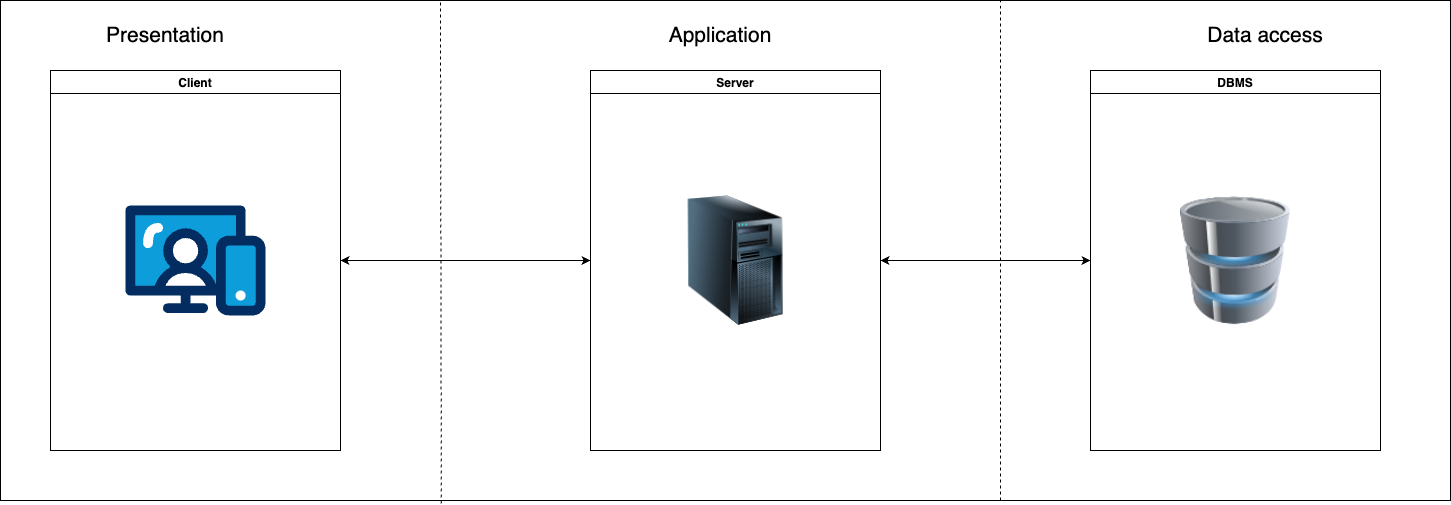
\includegraphics[width=\textwidth]{Images/three_tier.png}
    \caption{High level components and their interaction}
\end{figure}

The three-tier architecture was chosen for this type of system because of the several advantages it offers compared to other types of architectures. For what concerns scalability, it allows for easy scalability by separating the presentation, application, and data layers. Each layer can be scaled independently, allowing for better performance and resource utilization.
For what concers modulatiry, it promotes the separation of concers by dividing the system into distinct layers. This makes it easier to develop, test, and maintain each layer separately, improving overall code quality and reusability. The sepatarion of concerns also improves the maintainability of the system by providing clear boundaries between layers it makes easier to understand and modify specific parts of the system without affecting other layers.
The last advantage for which this architecture was chosen is flexibility. The three-tier provides flexibility in terms of technology choices. Each layer can be implemented using different technologies, allowing for the use of the most suitable tools and frameworks for each specific layer.

\begin{figure}[H]
    \centering
    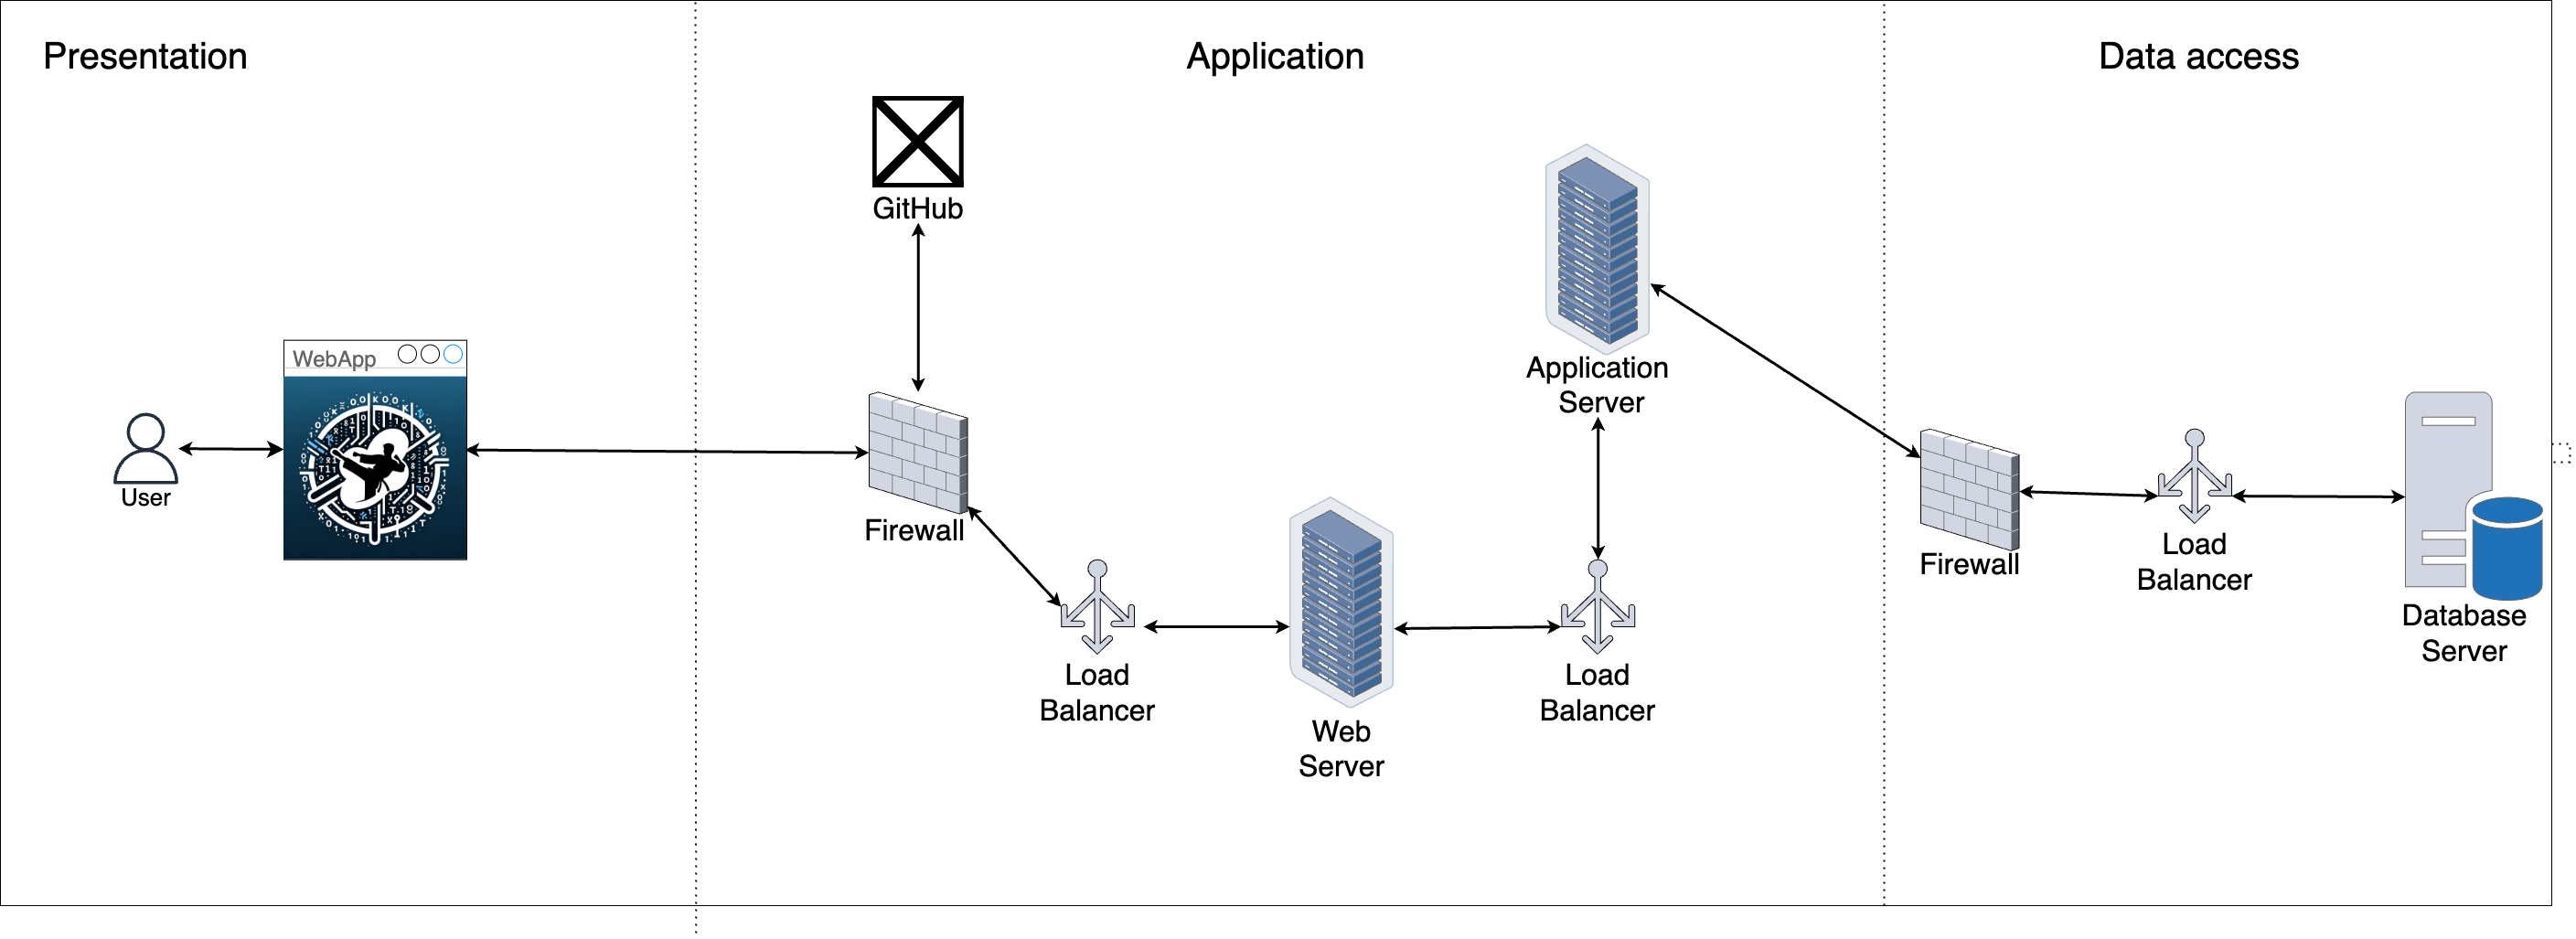
\includegraphics[width=\textwidth]{Images/high_level.png}
    \caption{High level system with interactions between the components}
    \label{fig:high_level_system}
\end{figure}

In the figure Figure\ \ref{fig:high_level_system} is shown the high level system with the interactions between the components. 
At the forefront is the Presentation layer, where a user engages with the web application through a web browser.
The web application depending on user interactions requests data from the web server. The interaction between the two is not direct since there is a firewall (for security reasons) and also a load balancer.

Moving inward, the Application layer serves as the system's operational core, where a network firewall establishes the first line of defense, safeguarding the internal processes. A load balancer stands right behind the firewall, directing incoming traffic to maintain system efficiency and reliability. This layer is further composed by an application server that executes the business logic, interfacing with databases or other external services as needed. Additionally, the presence of an upward arrow connecting the load balancer to GitHub to handle the evaluation trigger as well as the creation of the repositories. This is a very important feature of the system since it allows to automatically evaluate the students' submissions.

The final segment of the diagram is the Data Access layer, echoing the security and balance themes with its own firewall and load balancer, underscoring the system's commitment to secure data transactions. At the heart of this layer lies the database server, a robust storage solution that ensures data is efficiently stored, retrieved, and managed, completing the architecture's promise of a secure, scalable, and resilient web application environment.

\subsection{Component view}
In Figure\ \ref{fig:component_diagram} is shown the component diagram of the system. The system is divided into three main layers: presentation layer, application layer and data layer. The presentation layer is the interface between the user and the system and it is represented with the WebApp and Web Server Component. The application layer is the core of the CKB Platform and it is representend by the Application Server Subsystem. Finally the data layer is represented by the DBMS Component who is the only one that access the database.
\begin{figure}[H]
    \centering
    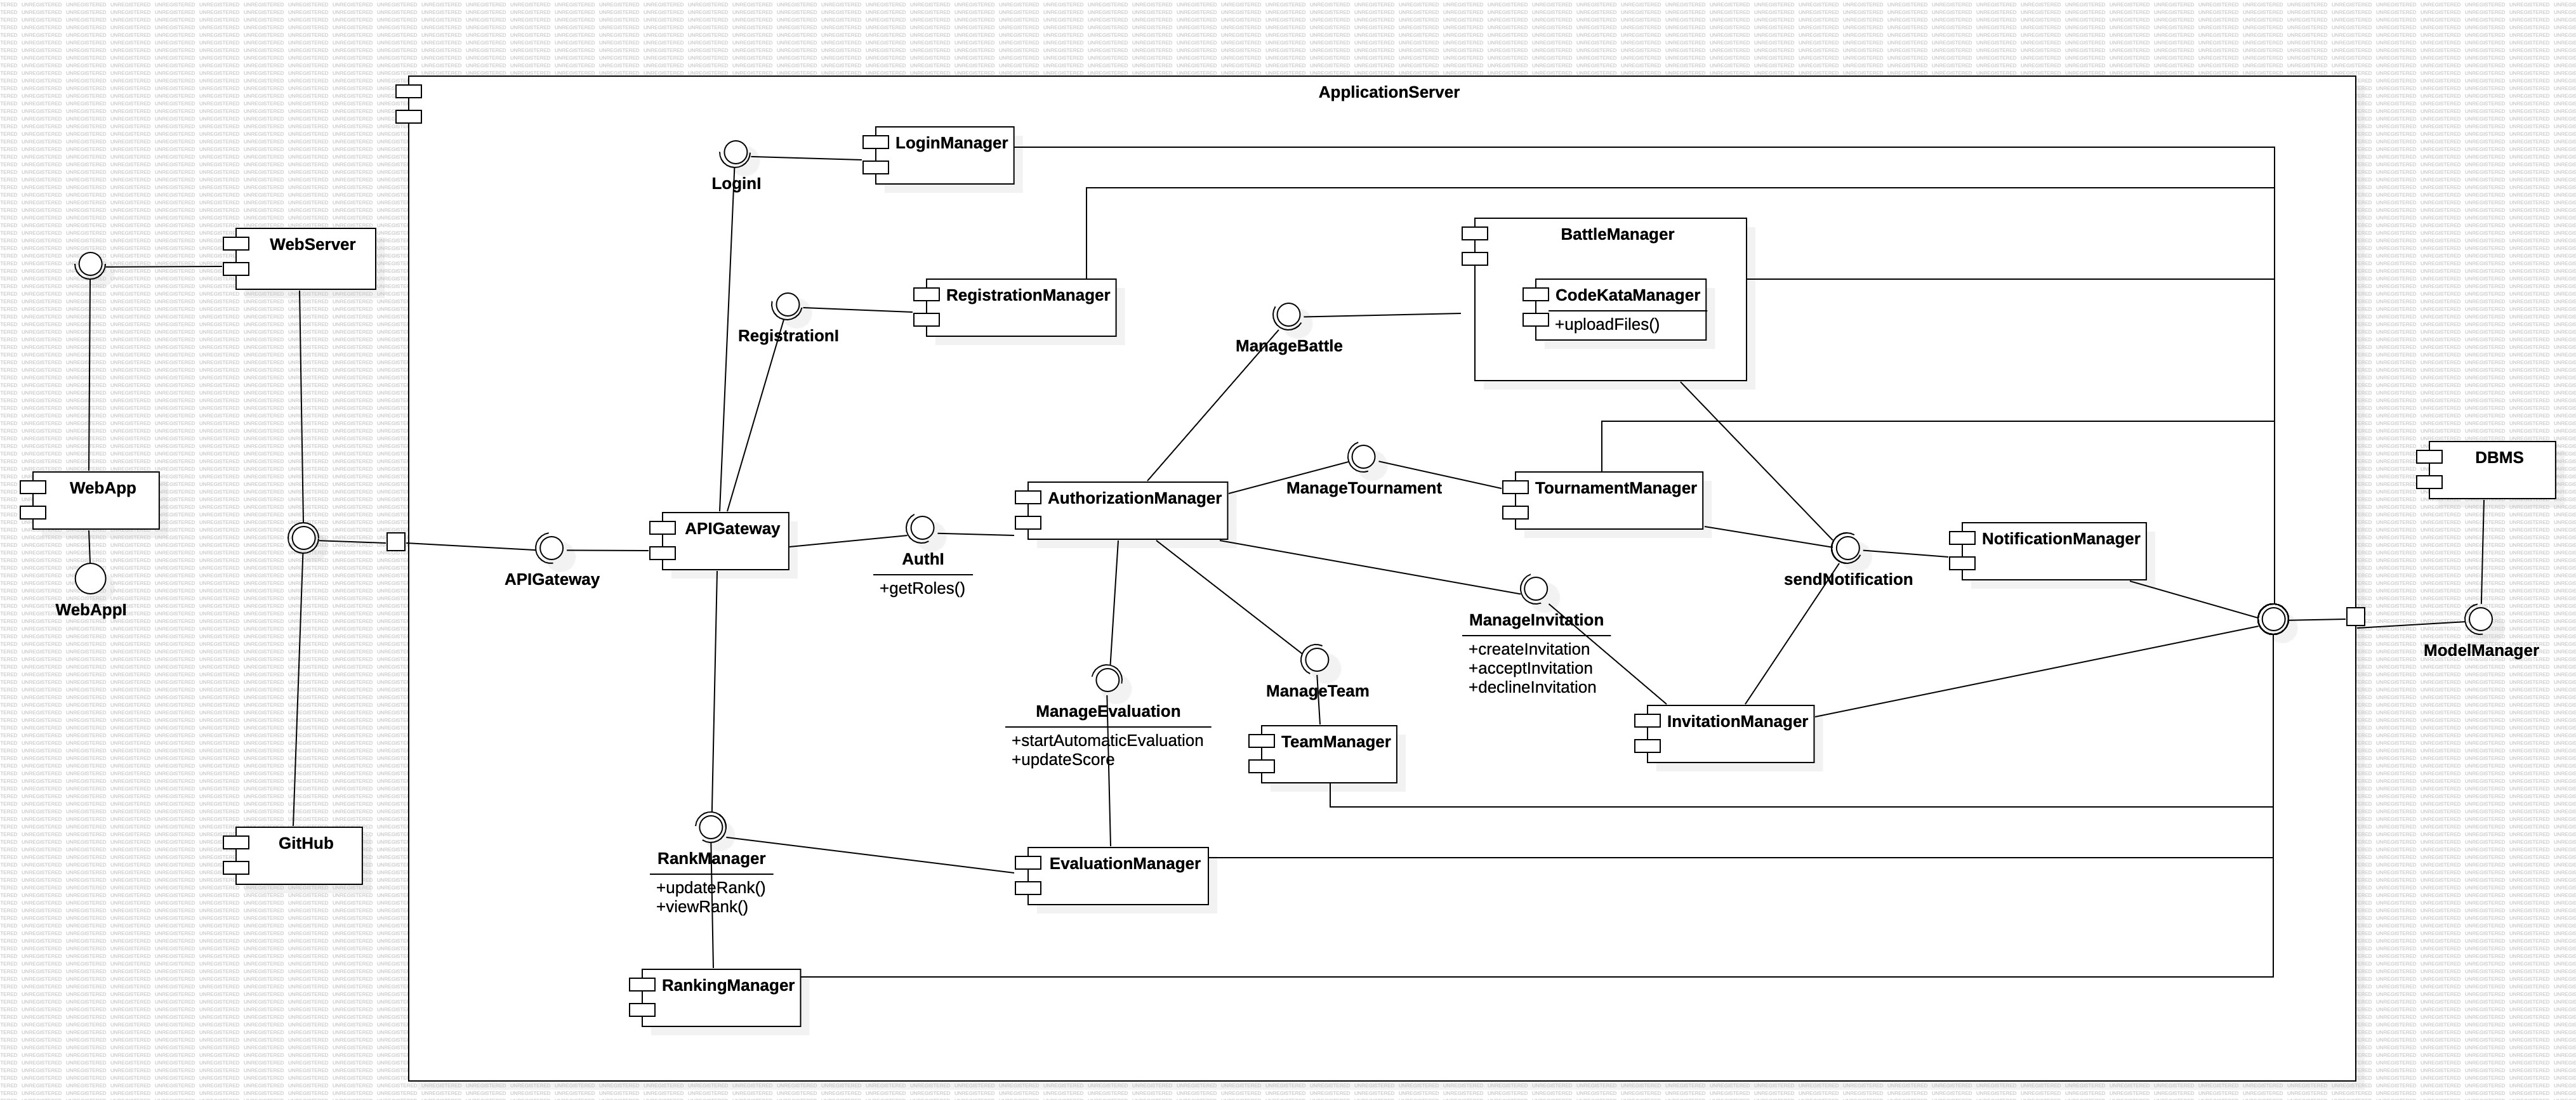
\includegraphics[angle=90,origin=c,width=0.6\textwidth]{Diagrams/ComponentDiagram.jpg}
    \caption{Component diagram}
    \label{fig:component_diagram}
\end{figure}
\clearpage
Regarding the presentation layer, it is represented by the following two components:
\begin{itemize}
    \item \textbf{WebApp}: it is the web application that the user interacts with. It is responsible for the presentation of the data and the interaction with the user. Since it communicates only with the Web Server, it can be executed by any device that has a web browser.
    \item \textbf{Web Server}: it is the component that handles the requests from the WebApp and forwards them to the Application Server. It is responsible to direct the requests to the APIGateway. It is also responsible to forward responses from the Application Server to the WebApp.
\end{itemize}
Regarding the application layer, it is represented by the components inside the Application Server Subsystem:
\begin{itemize}
    \item \textbf{APIGateway}: it is the component that handles the incoming requests to the Application Server. It is responsible to direct the requests to the correct component inside the Application Server Subsystem. It is also responsible to forward responses from the Application Server to the Web Server.
    \item \textbf{Login Manager}: it is the component that handles the login requests. It is responsible to check the credentials and to log the user in.
    \item \textbf{Registration Manager}: it is the component that handles the registration requests. It is responsible to create a new user.
    \item \textbf{Authorization Manager}: it is the component that handles the authorization requests. It is responsible to check if the user is authorized to perform the requested action. This is of paramount importance since only a user with Educator role can perform administrative actions, such as the creation of a new Tournament or Battle.
    \item \textbf{Evaluation Manager}: it is the component that handles the evaluation requests. It is responsible to evaluate the submissions of the students and to return the results. It performs the evaluation by running and testing the submissions provided by the students. It can be used also by the Educator to re-evaluate the submissions manually.
    \item \textbf{Ranking Manager}: it is the component that handles the rank of students in a Tournament.
    \item \textbf{Team Manager}: it is the component that handles the creation of teams and the assignment of students to teams. It is also responsible to guarantee that the restrictions on the number of students per team, set by the Educator, are respected.
    \item \textbf{Submission Manager}: it is the component that handles the submission of the students. The submission is created when the GitHub Action is triggered by the push of the student in the Team repository. It interacts with the Evaluation Manager to get the evaluation of the submission.
    \item \textbf{Invitation Manager}: it is the component that handles the invitation of both Students and Educator. In the case of the Students it is responsible to manage the invitation to join a Team. In the case of the Educator it is responsible to manage the invitation to join a Tournament.
    \item \textbf{Notification Manager}: it is the component that handles the notification requests. It is responsible to send notifications to the users. Such notifications are sent respecting the conditions previously specified in the RASD document.
    \item \textbf{Battle Manager}: it is the component that handles the creation and the management of Battles by the Educator. It is a complex component since it embodies also the CodeKata Manager. Since it contains the CodeKata Manager, it is responsible to handle the CodeKata files uploaded by the Educator. It interacts with the GitHub Component to create the repositories for the Battles. It also handles the different Battle phases, by guaranteeing the deadline restrictions set by the Educator.
    \item \textbf{Tournament Manager}: it is the component that handles the creation and the management of Tournaments by the Educator. It is responsible to handle the different Tournament phases, by guaranteeing the deadline restrictions set by the Educator.
\end{itemize}
Regarding the data layer, it is represented by the following component:
\begin{itemize}
    \item \textbf{DBMS}: it is the component that handles the access to the database. It is responsible to store and retrieve the data from the database. It is the only component that can access the database.
\end{itemize}
\subsection{Deployment view}
In this section is shown the deployment diagram of the system. The diagram is divided into three main tier: the presentation tier, the application tier and the data tier. 
\begin{figure}[H]
    \centering
    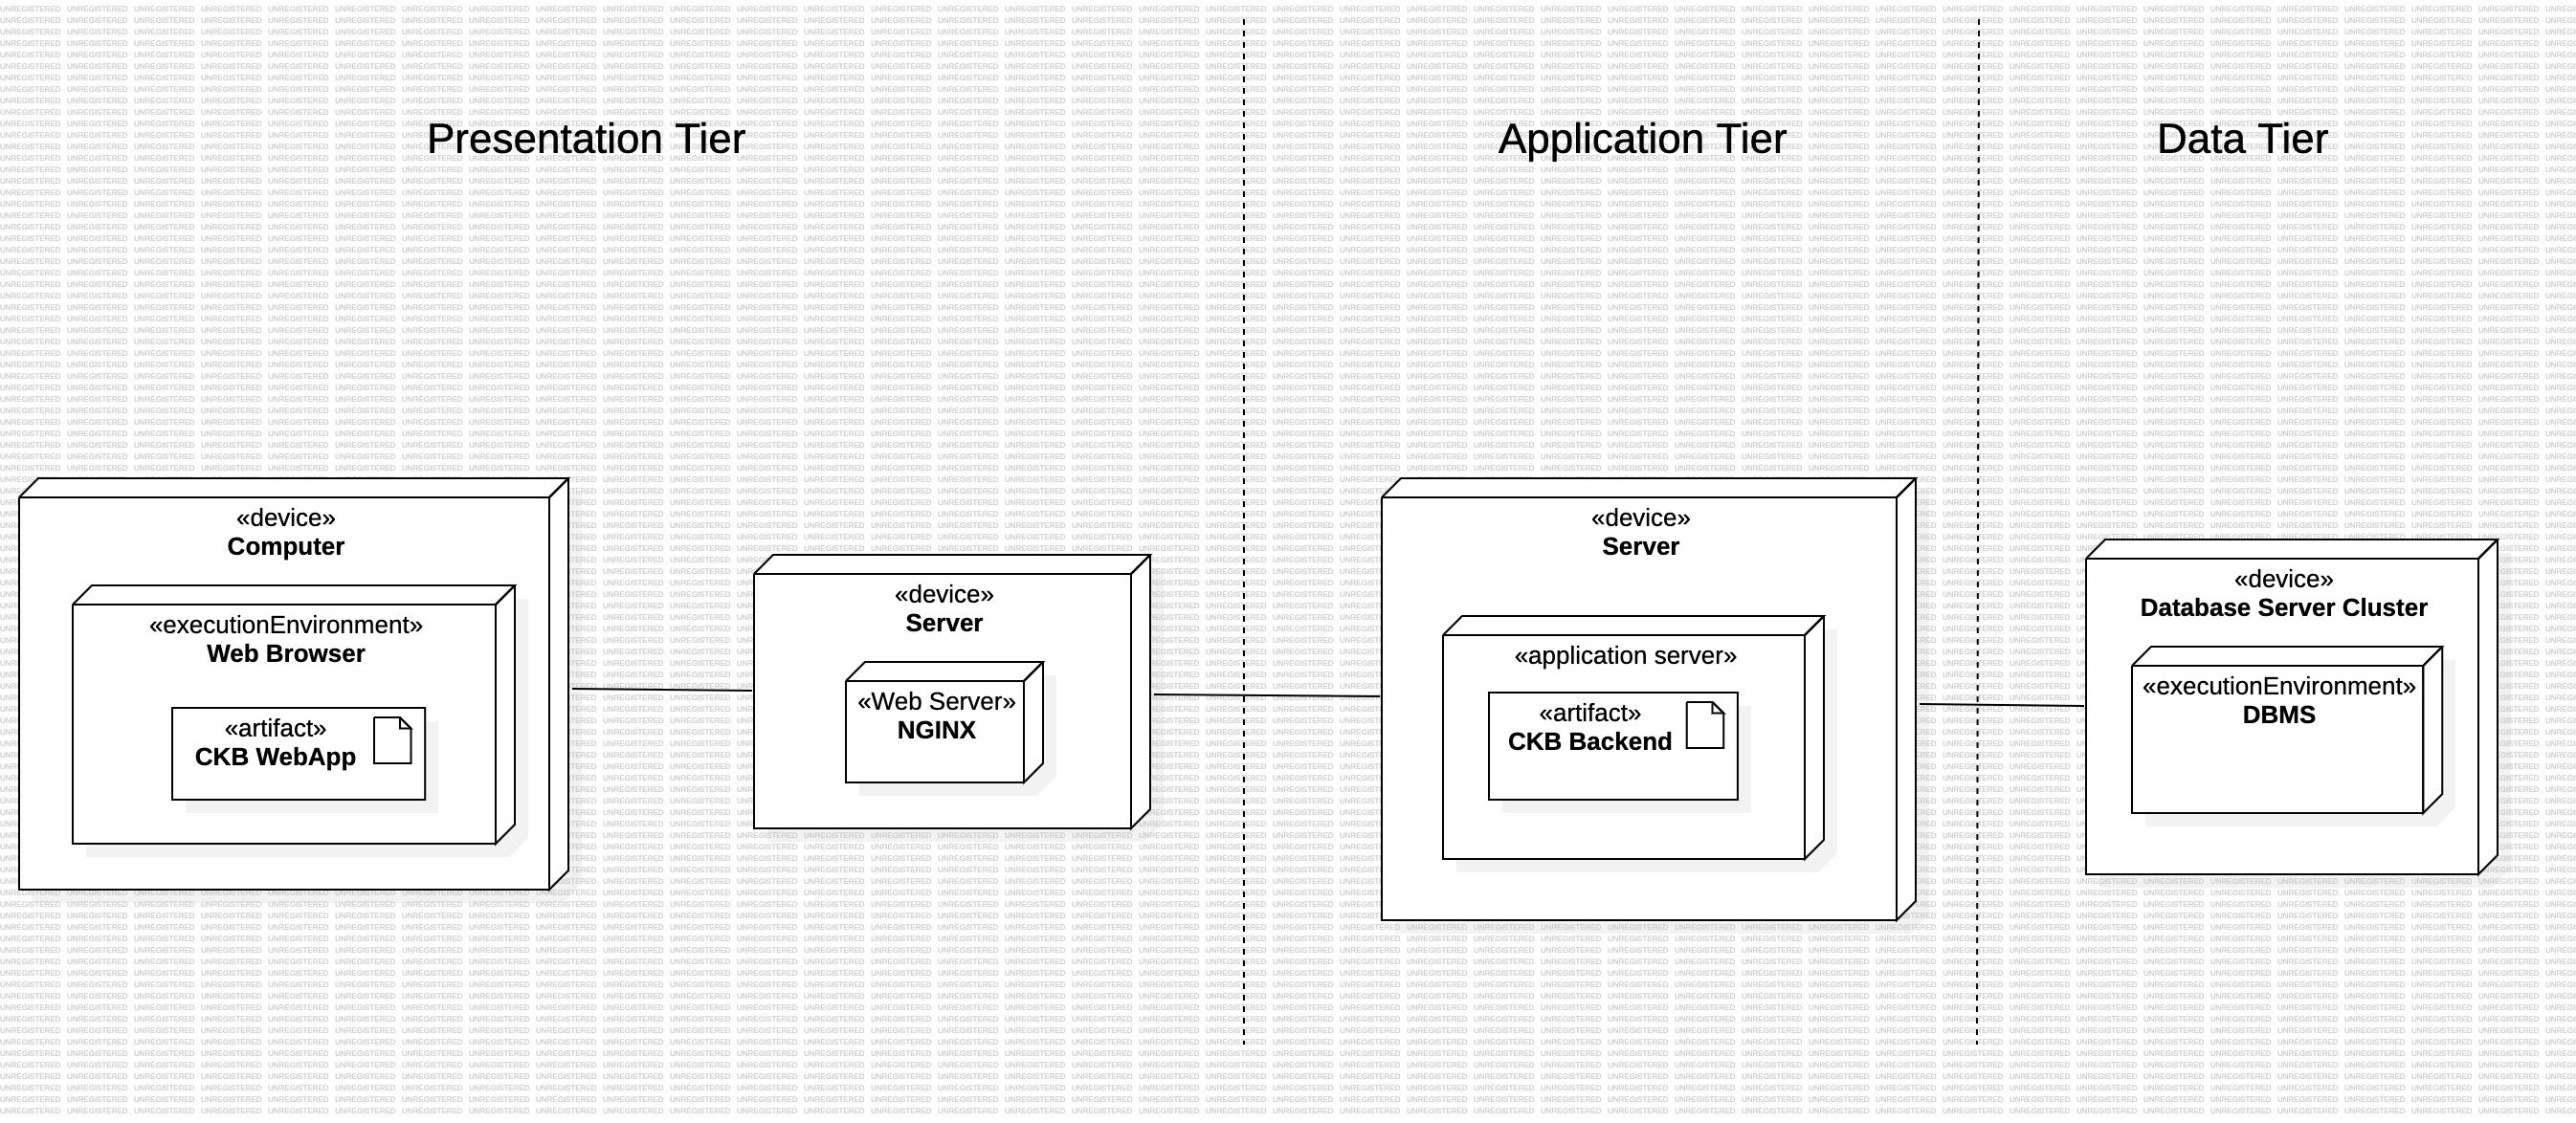
\includegraphics[width=\textwidth]{Diagrams/DeploymentDiagram.jpg}
    \caption{Deployment diagram}
    \label{fig:deployment_diagram}
\end{figure}
In figure Figure\ \ref{fig:deployment_diagram} is shown the deployment diagram of the system.
Regarding the presentation tier, it is represented by the following components:
\begin{itemize}
    \item \textbf{Computer}: it is a normal computer used by the user. It is the device that the user uses to interact with the CKB WebApp. It has no particular requirements since it only needs a web browser to access the WebApp.
    \item \textbf{Web Browser}: it is the software that the user uses to interact with the CKB WebApp. The CKB platform has to support the most common web browsers, such as Google Chrome, Mozilla Firefox, Microsoft Edge and Apple Safari.
    \item \textbf{CKB WebApp}: it is the web application that the user interacts with and it is used within the web browser. It is responsible for the presentation of the data and the interaction with the user.
    \item \textbf{Web Server}: it is a server that hosts a NGINX web server instance. The choice of NGINX is due to its high performance, low memory usage and high availability.
\end{itemize}
Regarding the application tier, it is represented by the following components:
\begin{itemize}
    \item \textbf{Application Server}: it is a server that hosts a CKB Backend application instance. It receives the requests from the Web Server and forwards it to the CKB Backend. At the same time it provides responses to the Web Server. It is also responsible to communicate with the DBMS to retrieve and store data.
    \item \textbf{CKB Backend}: it is the backend application of the CKB Platform. It handle the entire business logic of the application. It is responsible to process the forwarded requests and to provide responses to the Application Server.
\end{itemize}
Regarding the data tier, it is represented by the following components:
\begin{itemize}
    \item \textbf{Database Server Cluster}: it is a cluster of servers that hosts a DBMS instance. The choice of a cluster is due to the fact that it provides high availability and scalability. It is also responsible to guarantee the security of the data. It process the database specific requests sent by the Application Server.
    \item \textbf{DBMS}: it is the software that manages the database. It is responsible to store and retrieve the data from the database. It is the only component that can access the database.
\end{itemize}
\subsection{Component interfaces}

\textbf{Interface} LoginManager:
\begin{itemize}
    \item \texttt{Session login(String username, String password);}
    \item \texttt{void logout(Session session);}
\end{itemize}

\textbf{Interface} RegistrationManager:
\begin{itemize}
    \item \texttt{boolean register(UserDetails userDetails);}
\end{itemize}

\textbf{Interface} AuthorizationManager:
\begin{itemize}
    \item \texttt{List<Role> getRoles(User user);}
    \\ Get the roles of a user. The roles are used to determine if a user is authorized to perform a specific action.
\end{itemize}

\textbf{Interface} BattleManager:
\begin{itemize}
    \item \texttt{Battle createBattle(BattleDetails details);}
    \\ Create a new Battle. The BattleDetails contains all the information needed to create a new Battle.
    \item \texttt{boolean uploadFiles(Battle battle, CodeKata files);}
    \\ Upload the files of the CodeKata. The files must contain the tests and the automation scripts of the CodeKata.
    \item \texttt{boolean updateBattle(Battle battle, BattleDetails details);}
    \\ Updates the details of a Battle, such as the different stages and the deadlines.
    \item \texttt{List<Team> getTeams(Battle battle);}
    \\ Get the teams of a Battle.
    \item \texttt{Battle getBattle(int battleId);}
    \\ Get a Battle given its id.
    \item \texttt{Tournament getTournamentAssociated(int battleId);}
    \\ Get the Tournament associated to a Battle given its id.
    \item \texttt{boolean subscribe(Battle battle, Student student);}
    \\ Subscribe a Student to a Battle.
\end{itemize}

\textbf{Interface} TournamentManager:
\begin{itemize}
    \item \texttt{Tournament createTournament(TournamentDetails details);}
    \\ Create a new Tournament. The TournamentDetails contains all the information needed to create a new Tournament.
    \item \texttt{boolean updateTournament(Tournament tournament, TournamentDetails details);}
    \\ Updates the details of a Tournament, such as the different stages and the deadlines.
    \item \texttt{Tournament getTournament(int tournamentId);}
    \\ Get a Tournament given its id.
    \item textttt{void addEducator(Tournament tournament, Educator educator);}
    \\ Add an Educator to a Tournament.
\end{itemize}

\textbf{Interface} InvitationManager:
\begin{itemize}
    \item \texttt{List<Invitation> getInvitation(User user);}
    \\ Get the invitations of a user.
    \item \texttt{boolean sendInvitation(User user, Tournament | Team);}
    \\ Send an invitation to a user. The invitation can be to join a Tournament, if the user is an Educator, or to join a Team, if the user is a Student.
    \item \texttt{boolean acceptInvitation(Invitation invitation);}
    \\ Accept an invitation sent by another user.
    \item \texttt{boolean declineInvitation(Invitation invitation);}
    \\ Decline an invitation sent by another user.
\end{itemize}

\textbf{Interface} RankingManager:
\begin{itemize}
    \item \texttt{void updateRank(Student student, Tournament tournament, int newRank);}
    \\ Update the rank of a Student in a Tournament. This method can only be used by users with Educator Role.
    \item \texttt{int viewRank(Student student, Tournament tournament);}
    \\ View the rank of a Student in a Tournament.
\end{itemize}

\textbf{Interface} SubmissionManager:
\begin{itemize}
    \item \texttt{Submission submit(Item item);}
    \\ Submit a solution to a Battle. The Item contains the code of the solution.
    \item \texttt{Item getSubmission(int submissionId);}
    \\ Get the code of a submission given its id.
    \item \texttt{SubmissionResult getSubmissionResult(int submissionId);}
    \\ Get the evaluation of a submission given its id.
    \item \texttt{Battle getBattleAssociated(int SubmissionID);}
    \\ Get the Battle associated to a submission given its id.
    \item \texttt{Team getTeamAssociated(int SubmissionID);}
    \\ Get the Team associated to a submission given its id.
    \item \texttt{Score updateScore(int SubmissionID);}
    \\ Update the score of a submission.
\end{itemize}

\textbf{Interface} EvaluationManager:
\begin{itemize}
    \item \texttt{int startAutomaticEvaluation(Submission submission);}
    \\ Start the automatic evaluation of a submission.
    \item \texttt{boolean updateSubmissionResult(SubmissionResult result);}
    \\ Update the evaluation of a submission. Used when an Educator manually re-evaluates a submission.
\end{itemize}

\textbf{Interface} EvaluationManager:
\begin{itemize}
    \item \texttt{boolean startAutomaticEvaluation(Submission submission);}
    \\ Start the automatic evaluation of a submission. This method is called by the GitHub Action when a new submission is pushed to the repository.
\end{itemize}

\textbf{Interface} NotificationManager:
\begin{itemize}
    \item \texttt{void notify(User user, Notification notification);}
    \\ Send a notification to a user.
\end{itemize}

\textbf{Interface} ModelManager:
\begin{itemize}
    \item \texttt{boolean saveModel(DataModel model);}
    \\ Save a DataModel in the database.
    \item \texttt{DataModel getModel(DataModel model, List<Filter> filters);}
    \\ Get a DataModel from the database given its id.
    \item \texttt{boolean updateModel(DataModel model);}
    \\ Update a DataModel in the database.
    \item \texttt{boolean deleteModel(DataModel model);}
    \\ Delete a DataModel from the database.
\end{itemize}

\textbf{Interface} TeamManager:
\begin{itemize}
    \item \texttt{Team createTeam(TeamDetails details);}
    \\ Create a new Team. The TeamDetails contains all the information needed to create a new Team.
    \item \texttt{boolean updateTeam(Team team, TeamDetails details);}
    \\ Updates the details of a Team, such as the name and the members.
    \item \texttt{boolean addMember(Team team, Student student);}
    \\ Add a Student to a Team.
    \item \texttt{Team getTeam(int teamId);}
    \\ Get a Team given its id.
    \item \texttt{List<Student> getMembers(Team team);}
    \\ Get the members of a Team.
\end{itemize}

\subsection{Runtime view}
In this section are shown the sequence diagrams of the main functionalities of the system previously described in the RASD document. Starting from the \textit{Component View} section of this document, it is possible to identify the components interactions that are shown in the following sequence diagrams.

\subsubsection*{Login}
\begin{figure}[H]
    \centering
    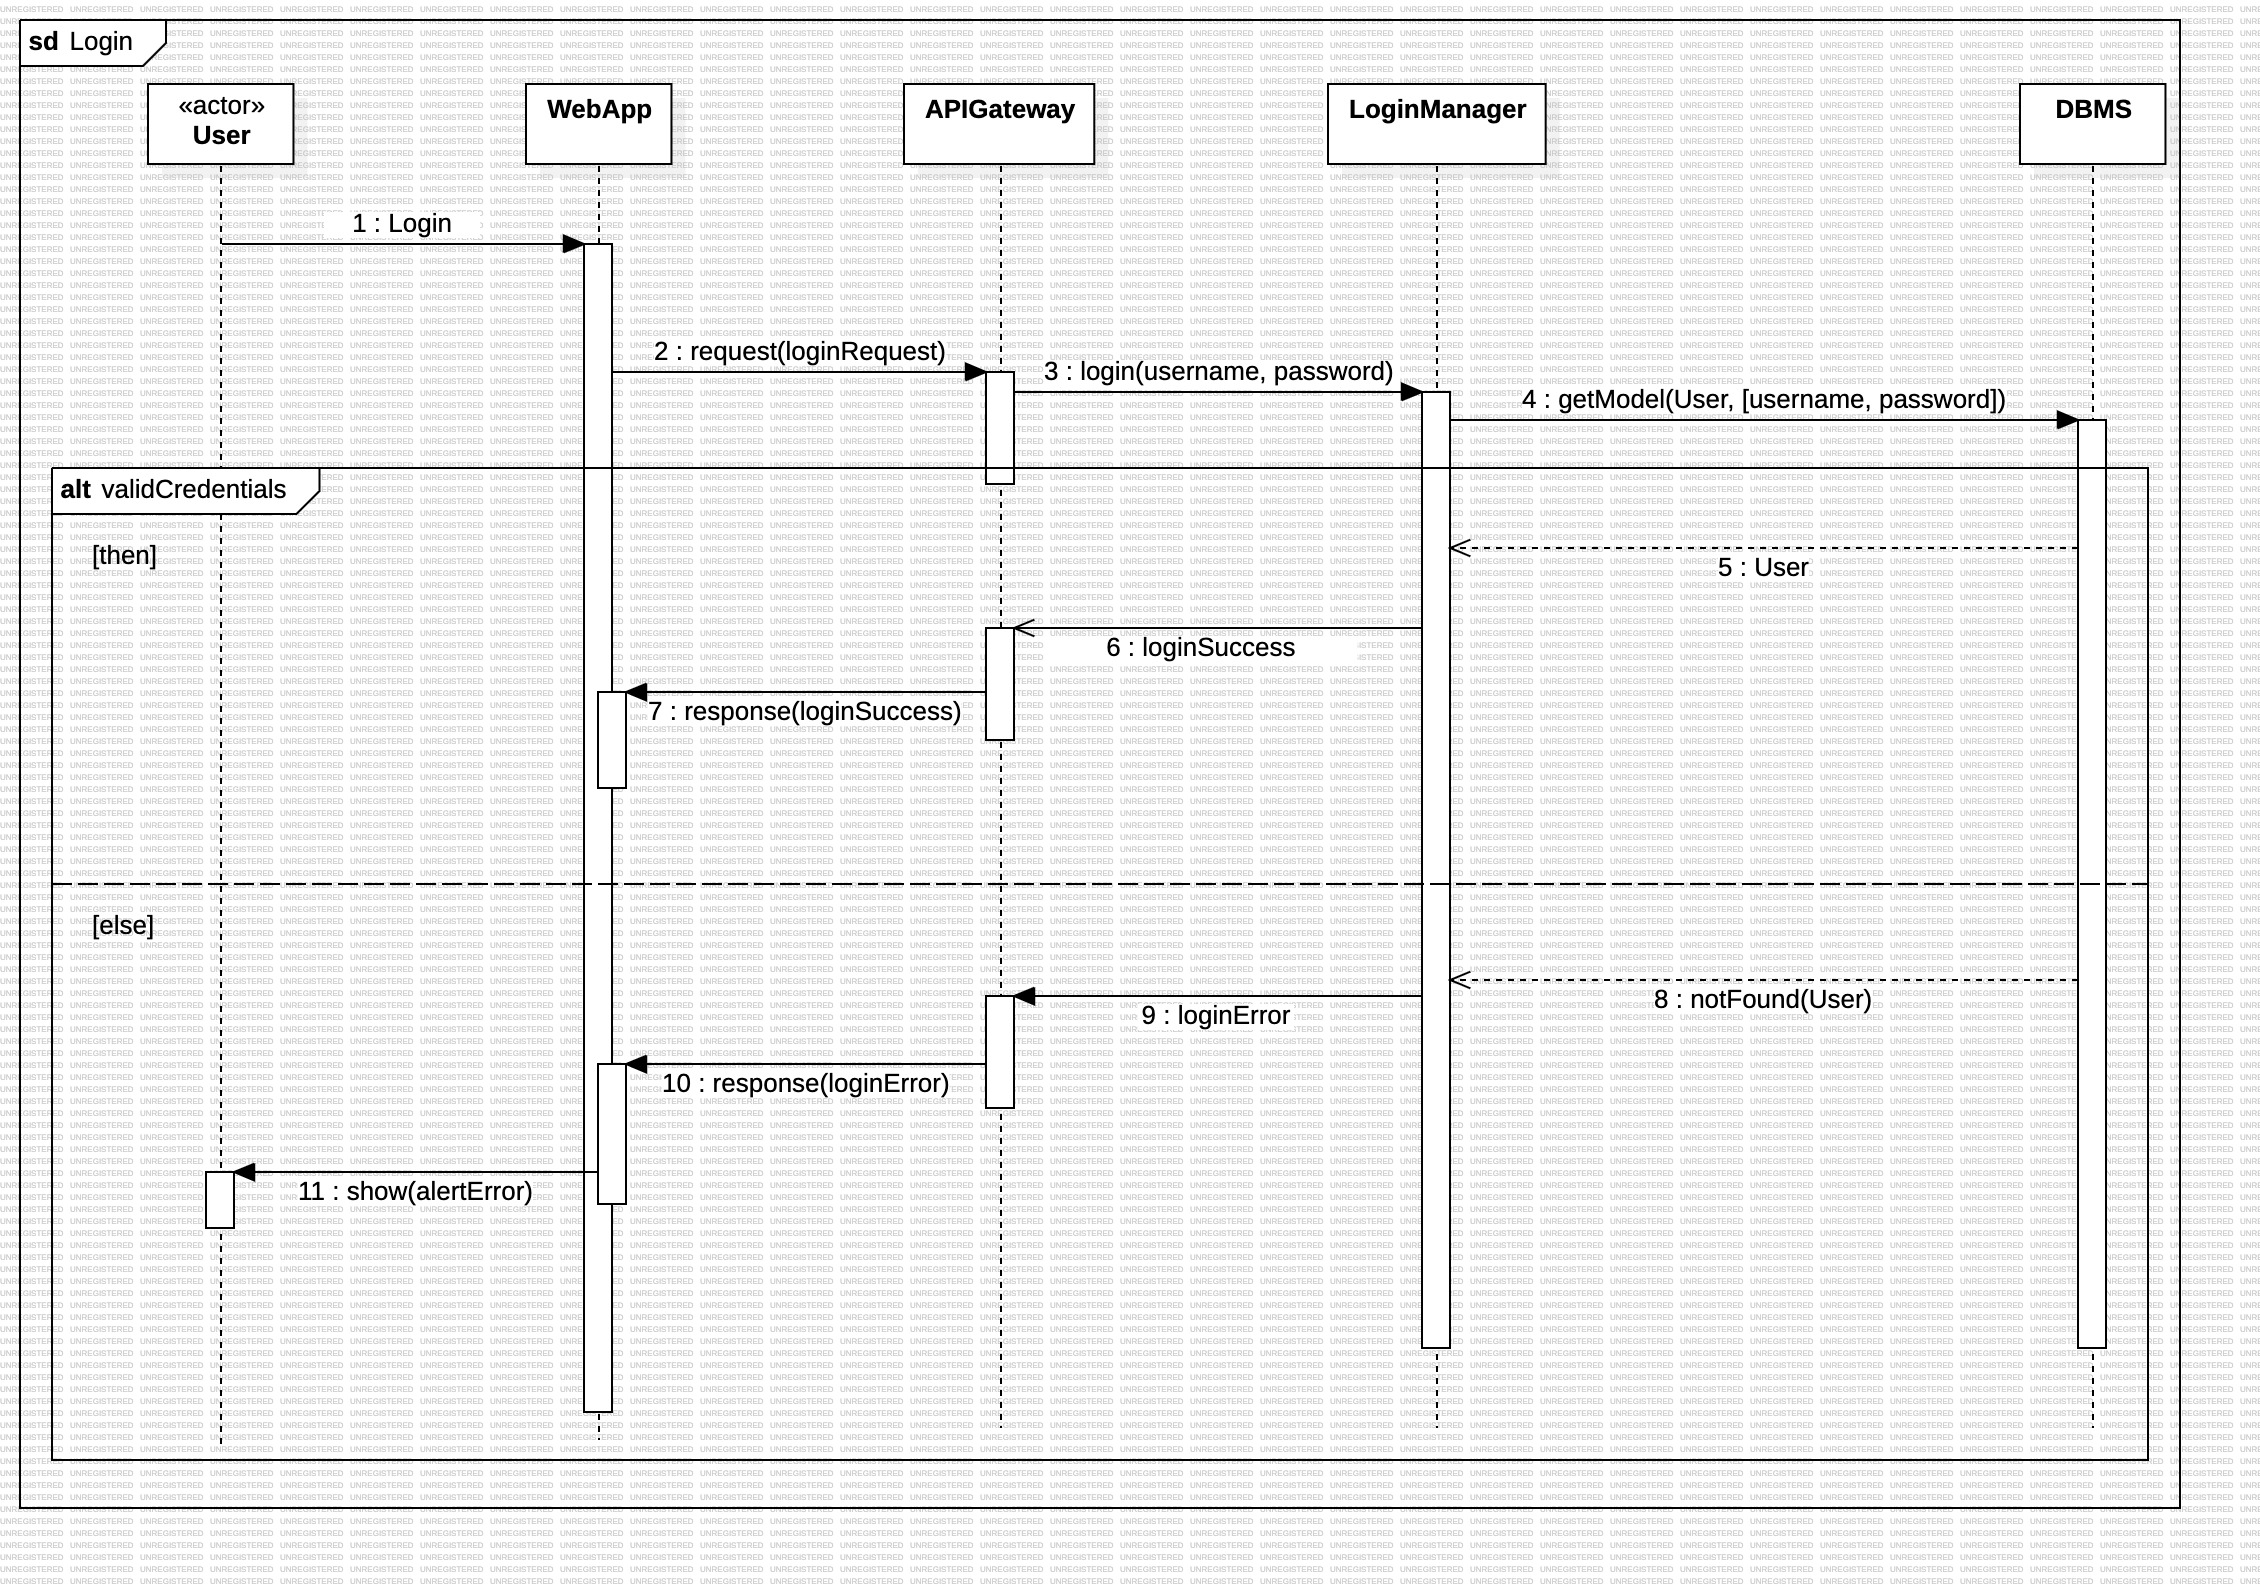
\includegraphics[width=\textwidth]{Diagrams/LoginSD.jpg}
    \caption{Runtime view Login}
    \label{fig:runtime_view_login}
\end{figure}
\subsubsection*{Creation of a tournament}
\begin{figure}[H]
    \centering
    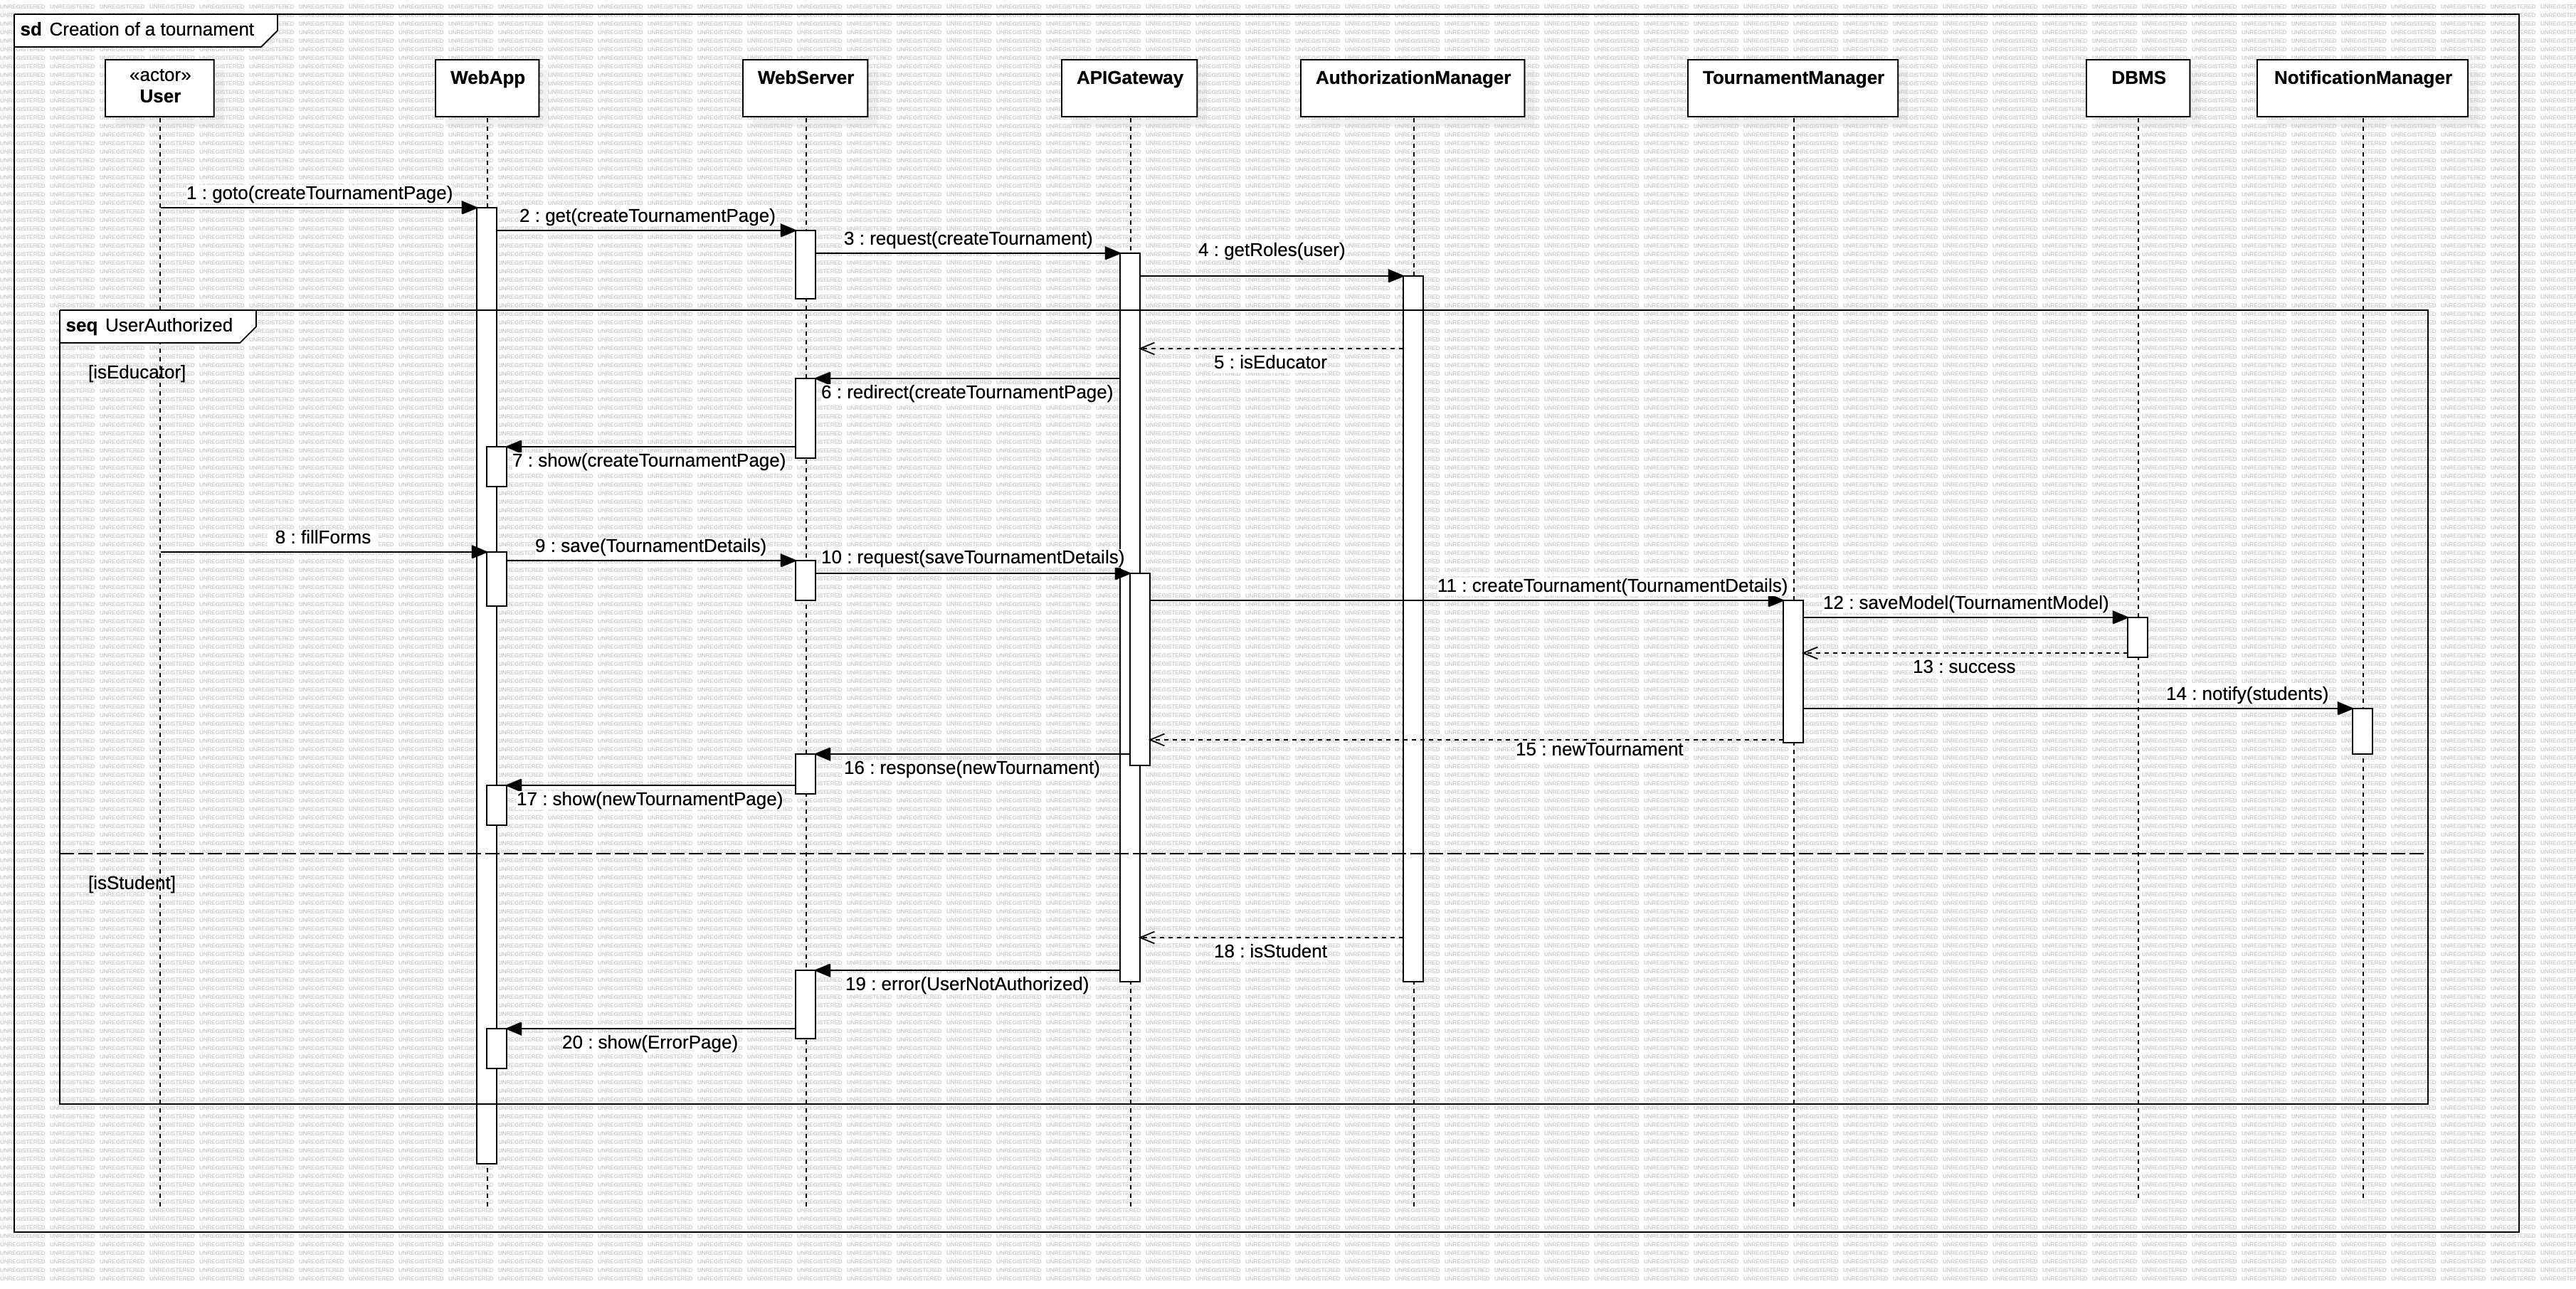
\includegraphics[width=\textwidth]{Diagrams/CreationTournamentSD.jpg}
    \caption{Runtime view Creation of a tournament}
    \label{fig:runtime_view_tournament_creation}
\end{figure}

\subsubsection*{Creation of a battle}
\begin{figure}[H]
    \centering
    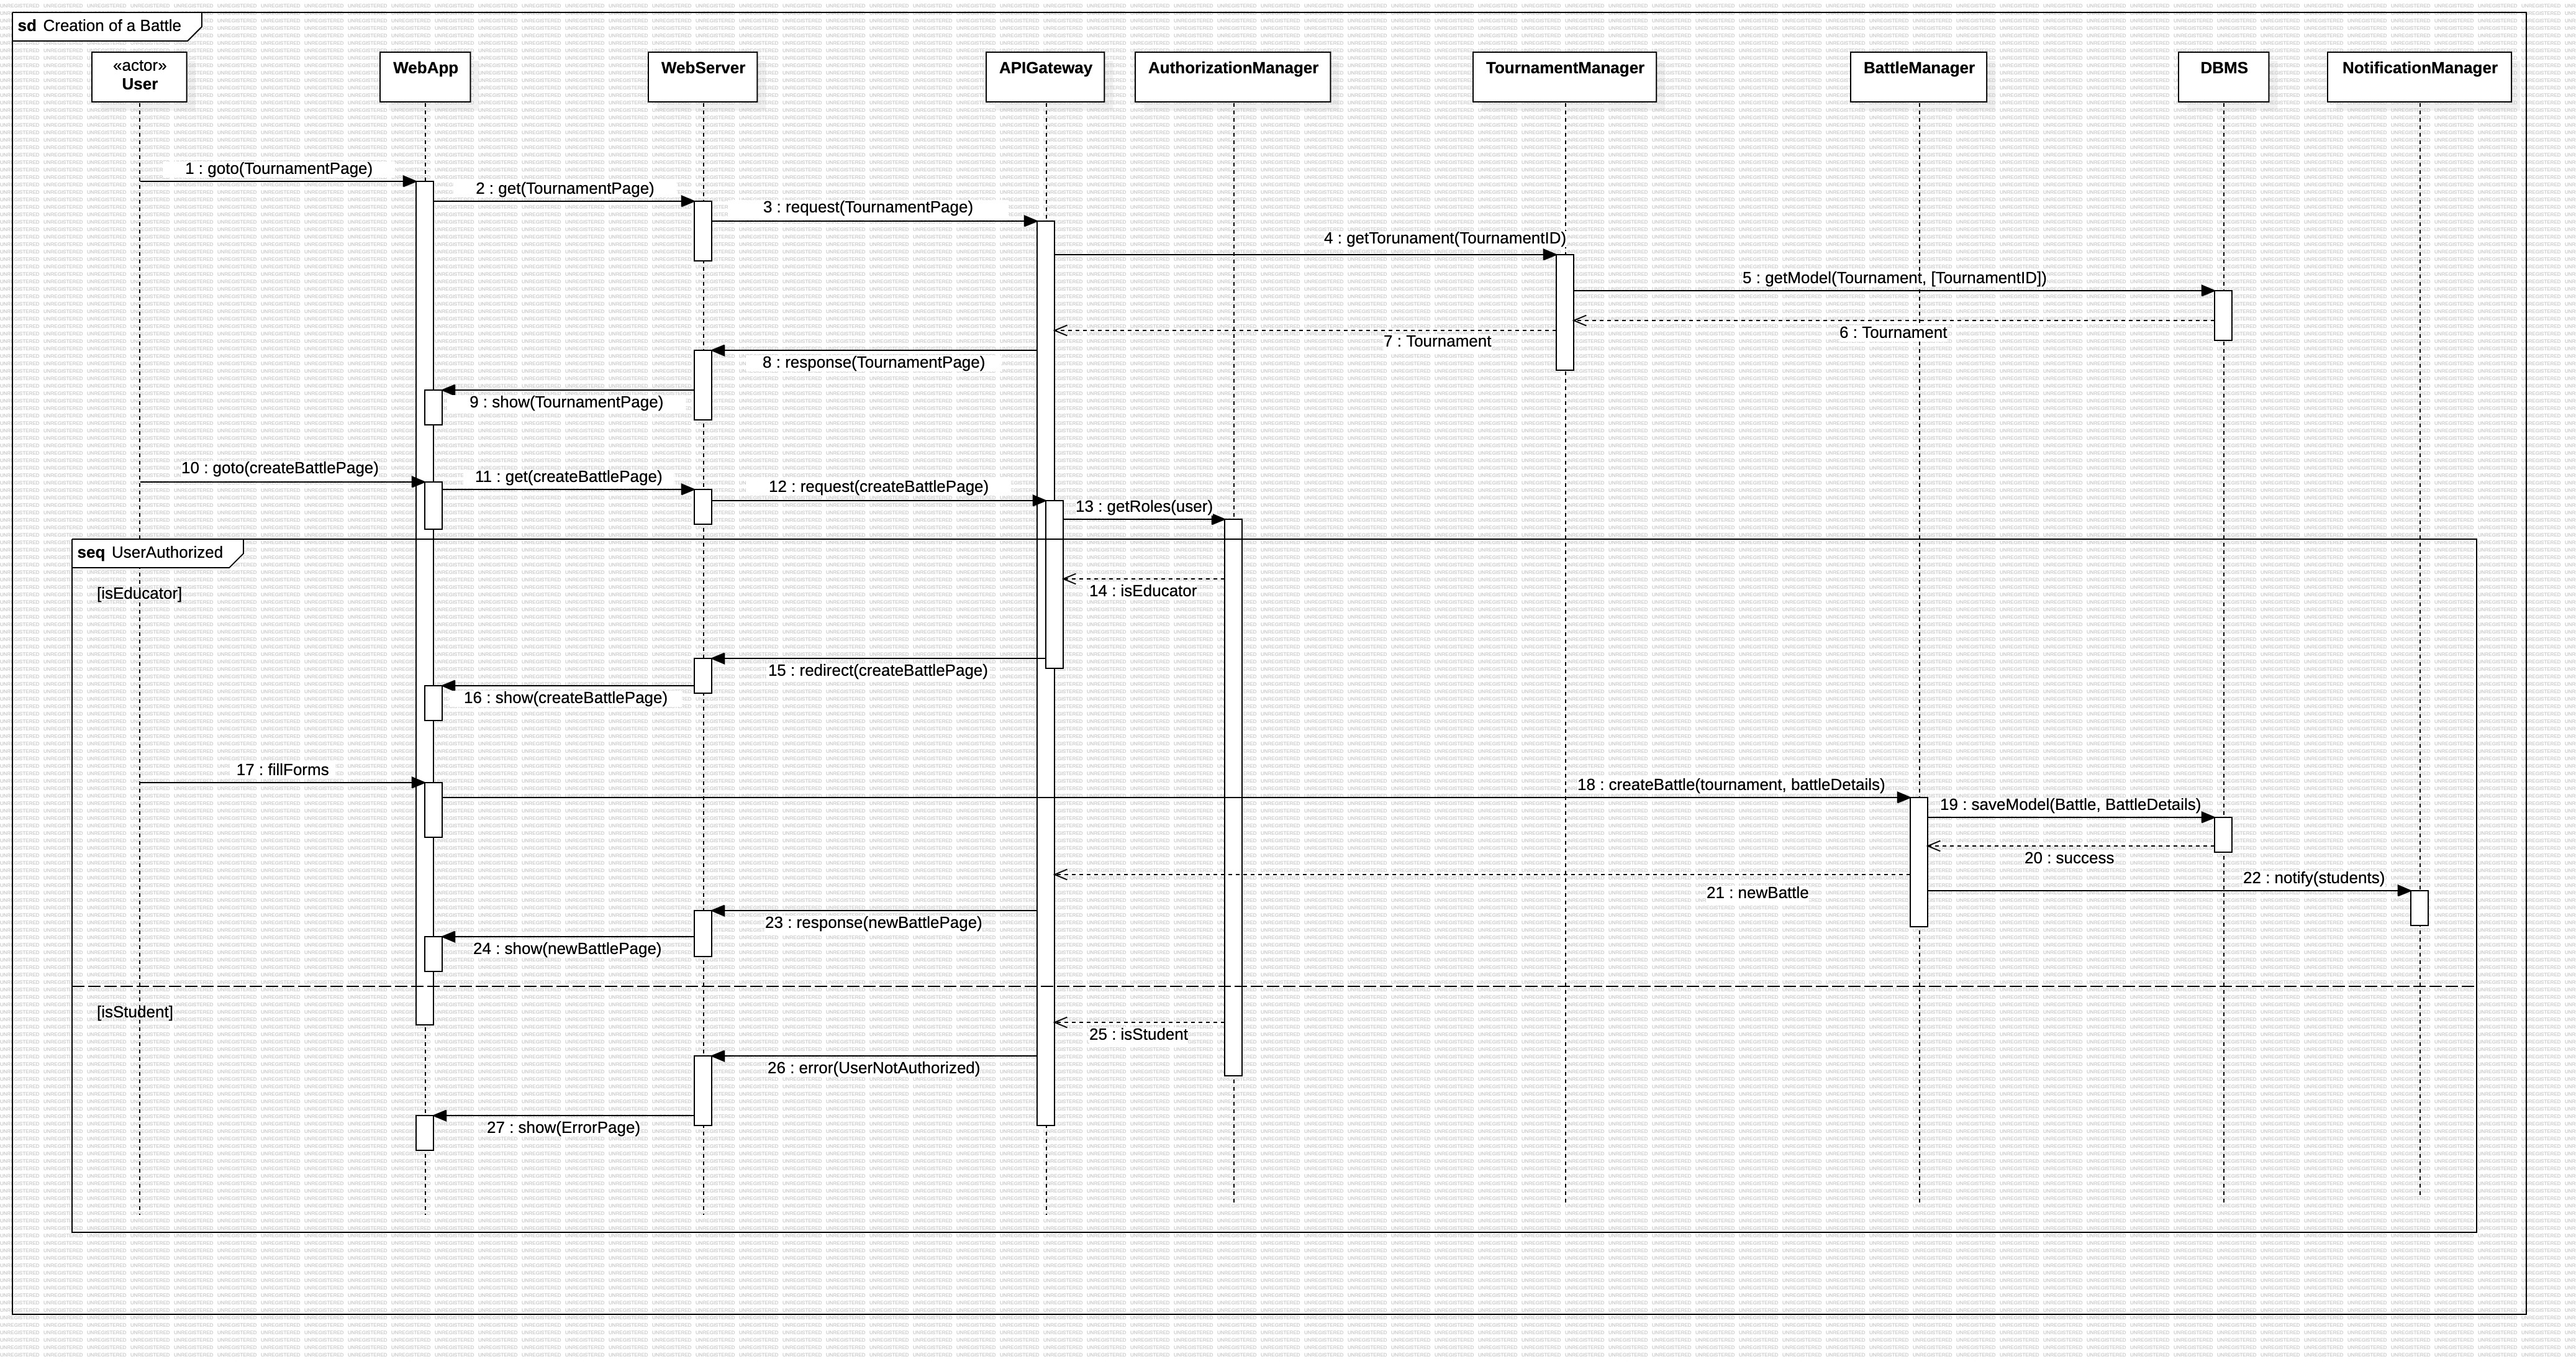
\includegraphics[width=\textwidth]{Diagrams/CreationBattleSD.jpg}
    \caption{Runtime view Creation of a battle}
    \label{fig:runtime_view_battle_creation}
\end{figure}
\subsubsection*{Invite other educators to a tournament}
\begin{figure}[H]
    \centering
    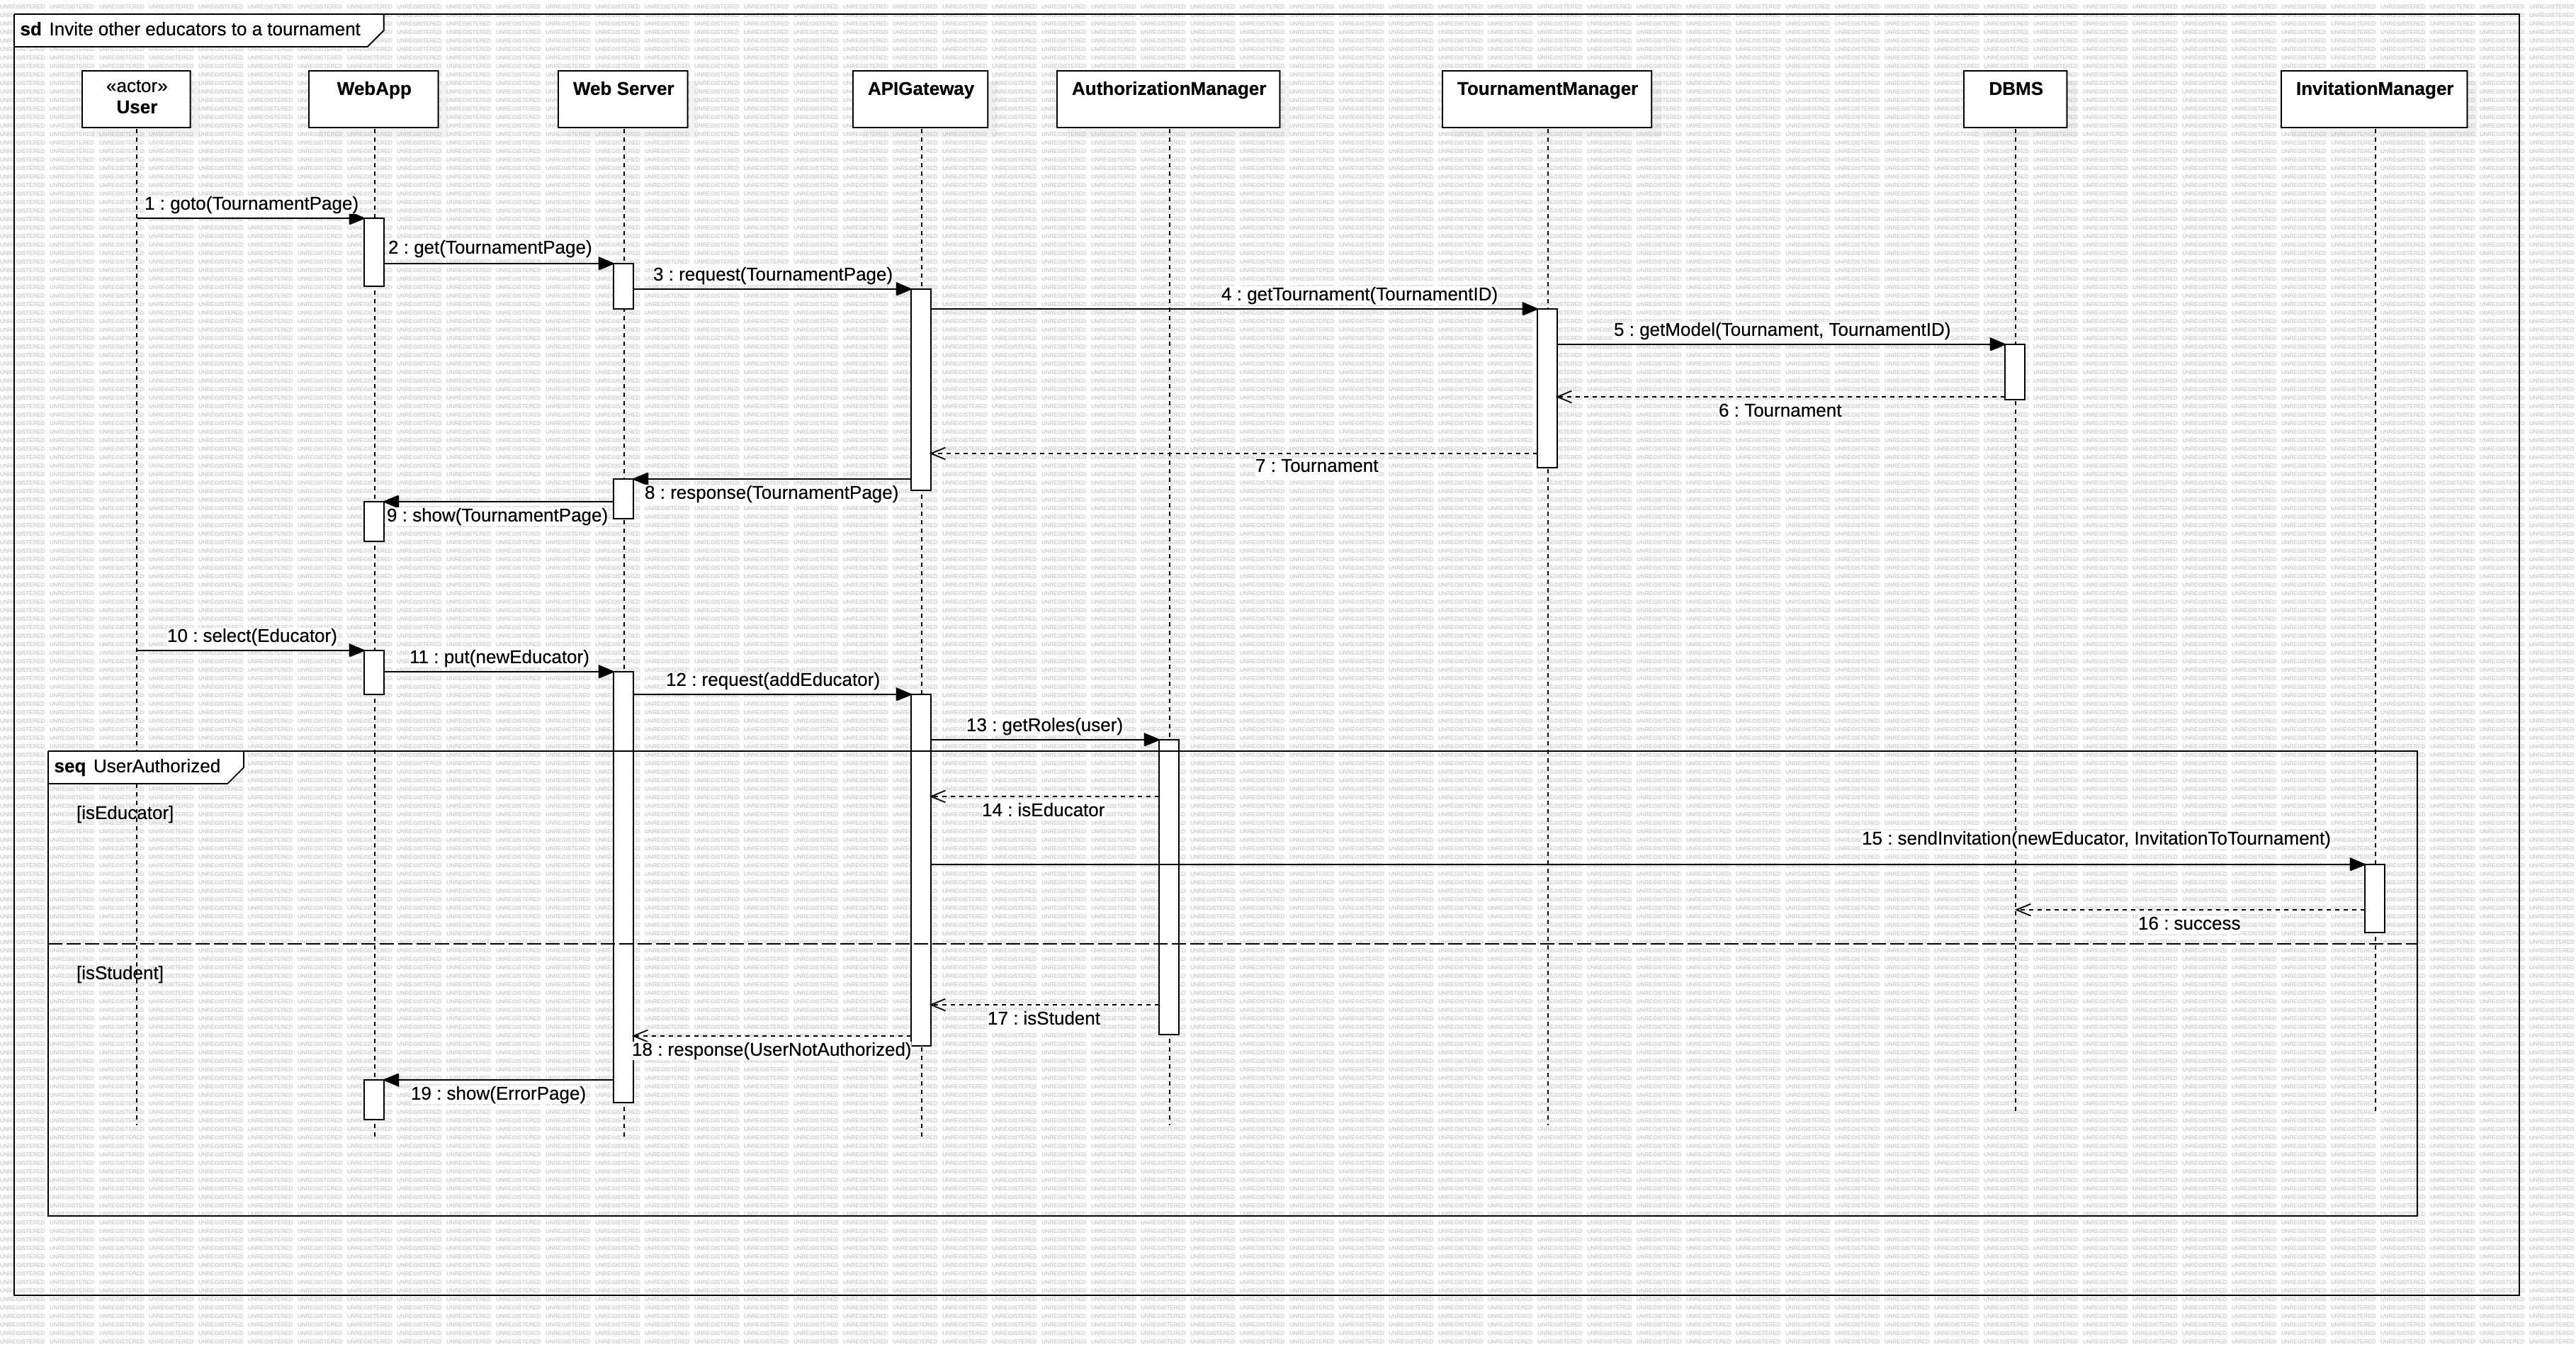
\includegraphics[width=\textwidth]{Diagrams/InviteEducatorSD.jpg}
    \caption{Runtime view Invite other educators to a tournament}
    \label{fig:runtime_view_invite_educator}
\end{figure}
\subsubsection*{Subscribe to a tournament}
\begin{figure}[H]
    \centering
    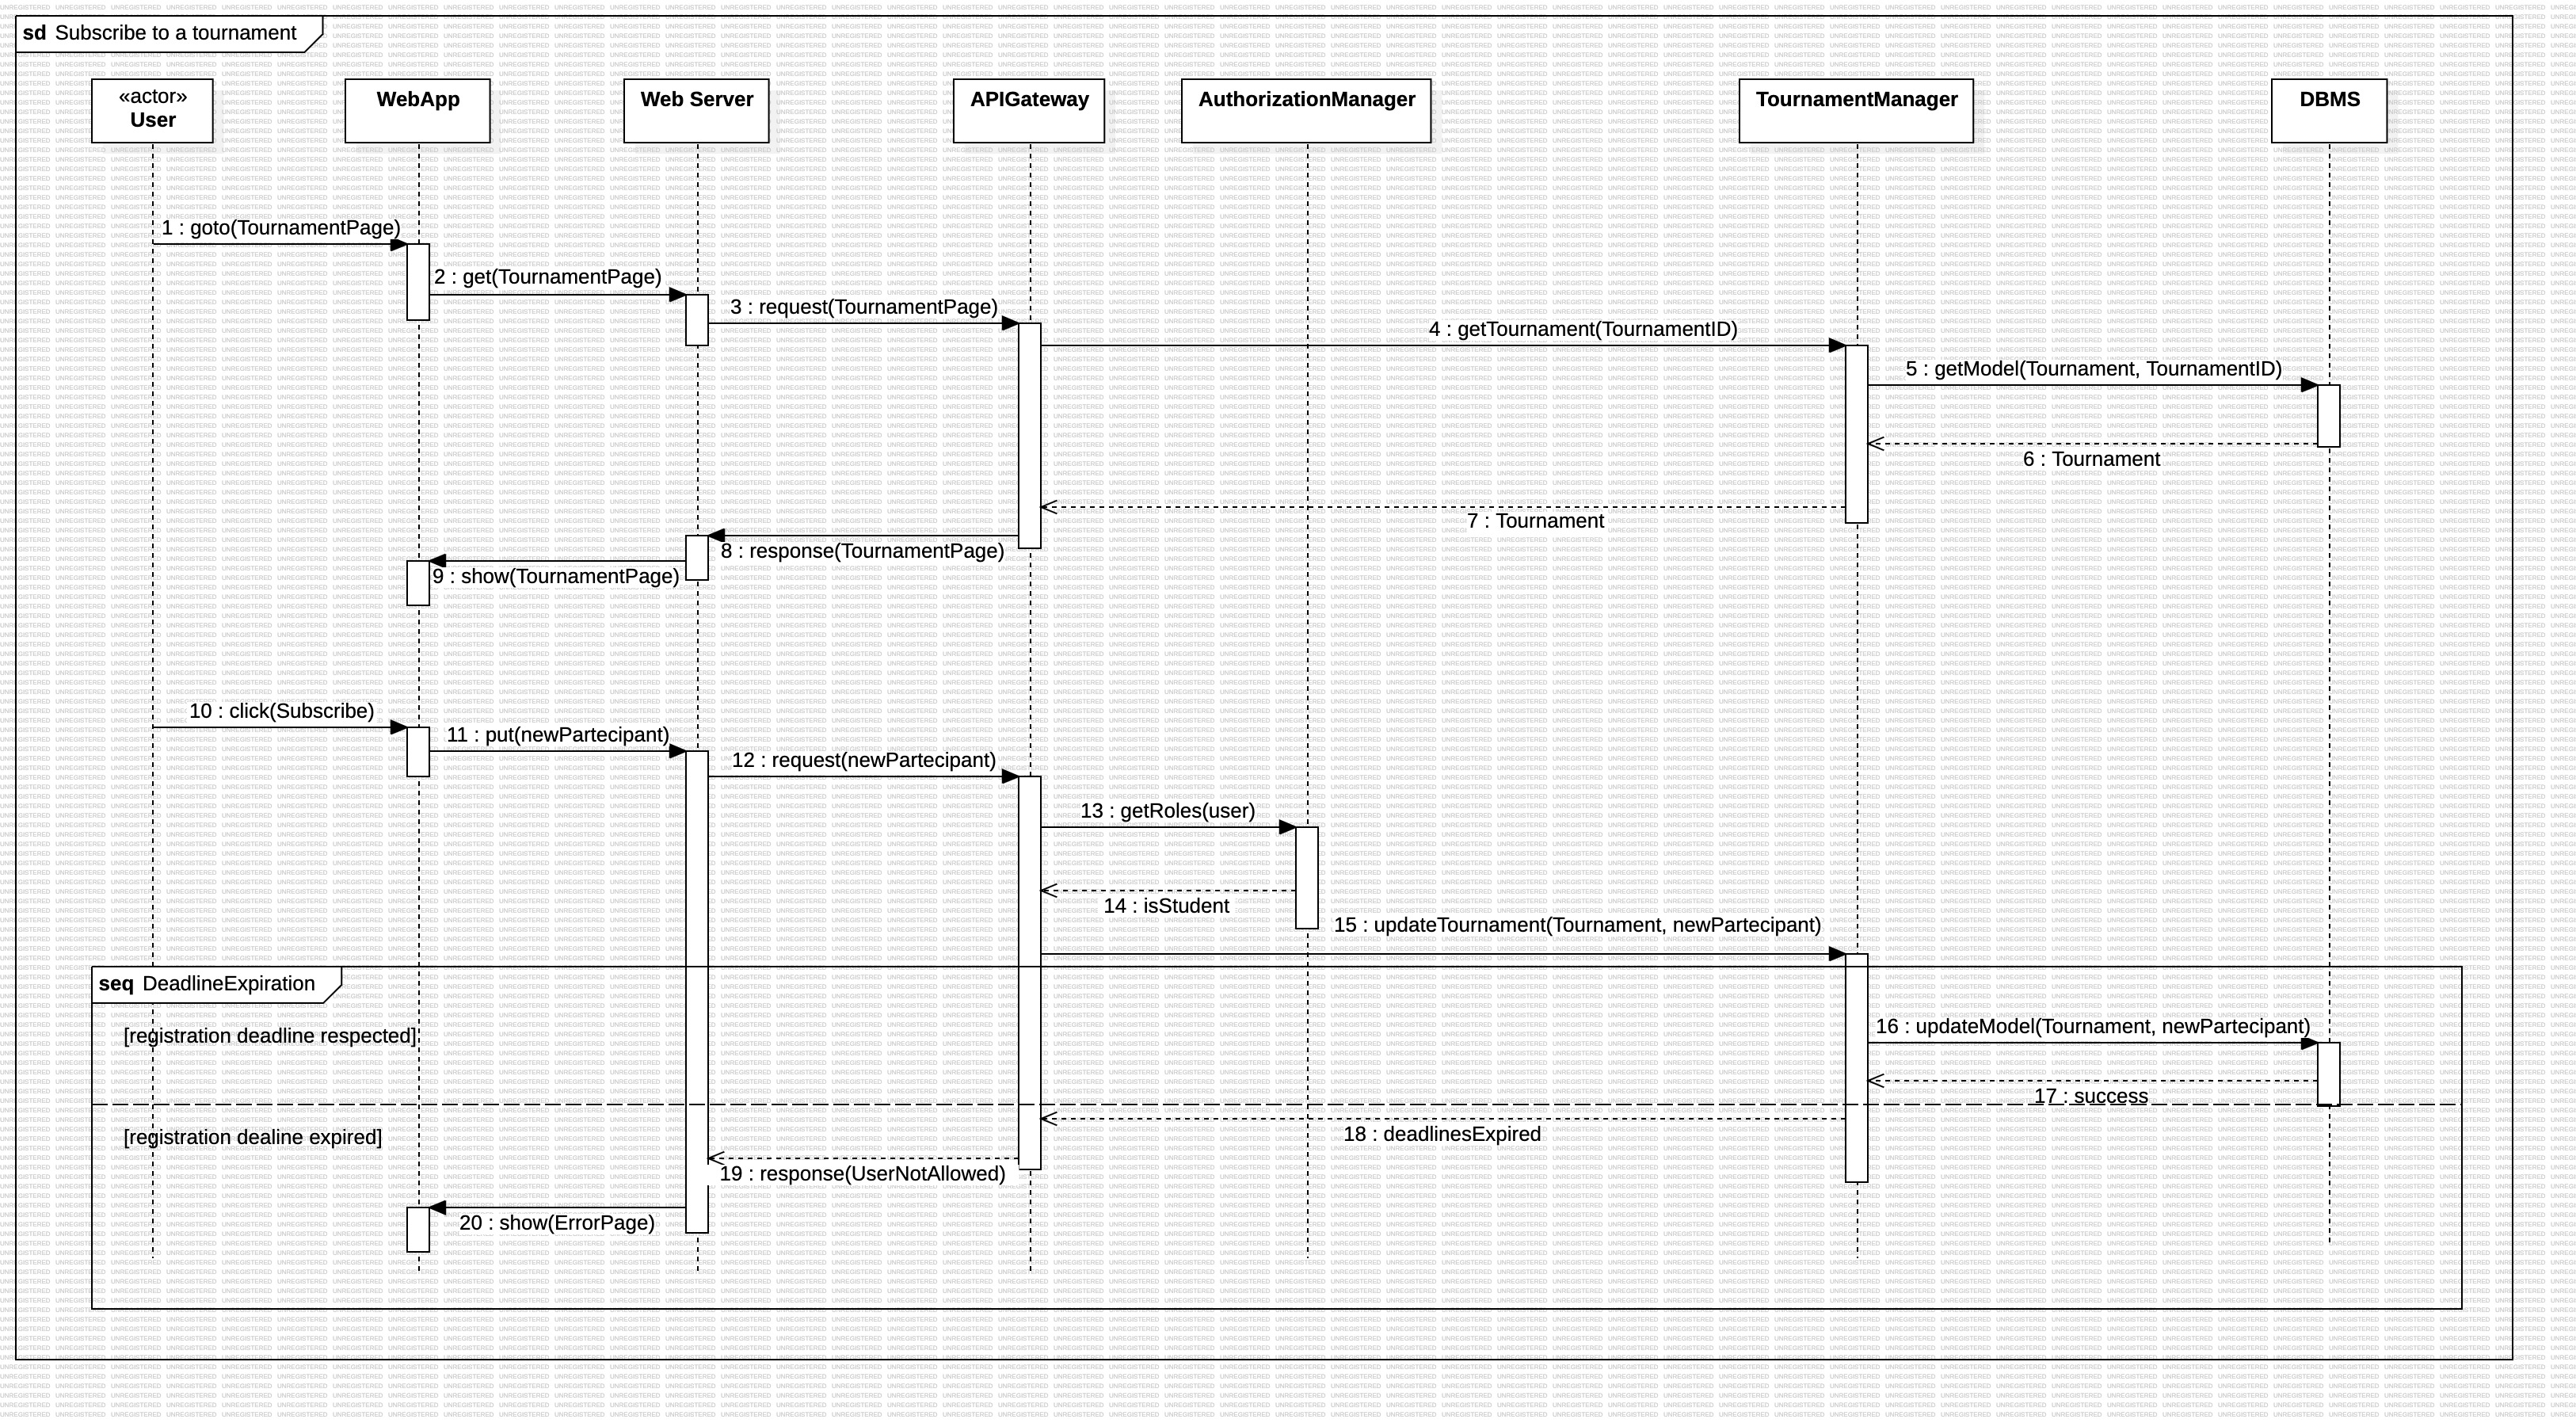
\includegraphics[width=\textwidth]{Diagrams/SubscribeTournamentSD.jpg}
    \caption{Runtime view Subscribe to a tournament}
    \label{fig:runtime_view_subscribe_tournament}
\end{figure}

\subsubsection*{Accept invitation to a team for a battle}
\begin{figure}[H]
    \centering
    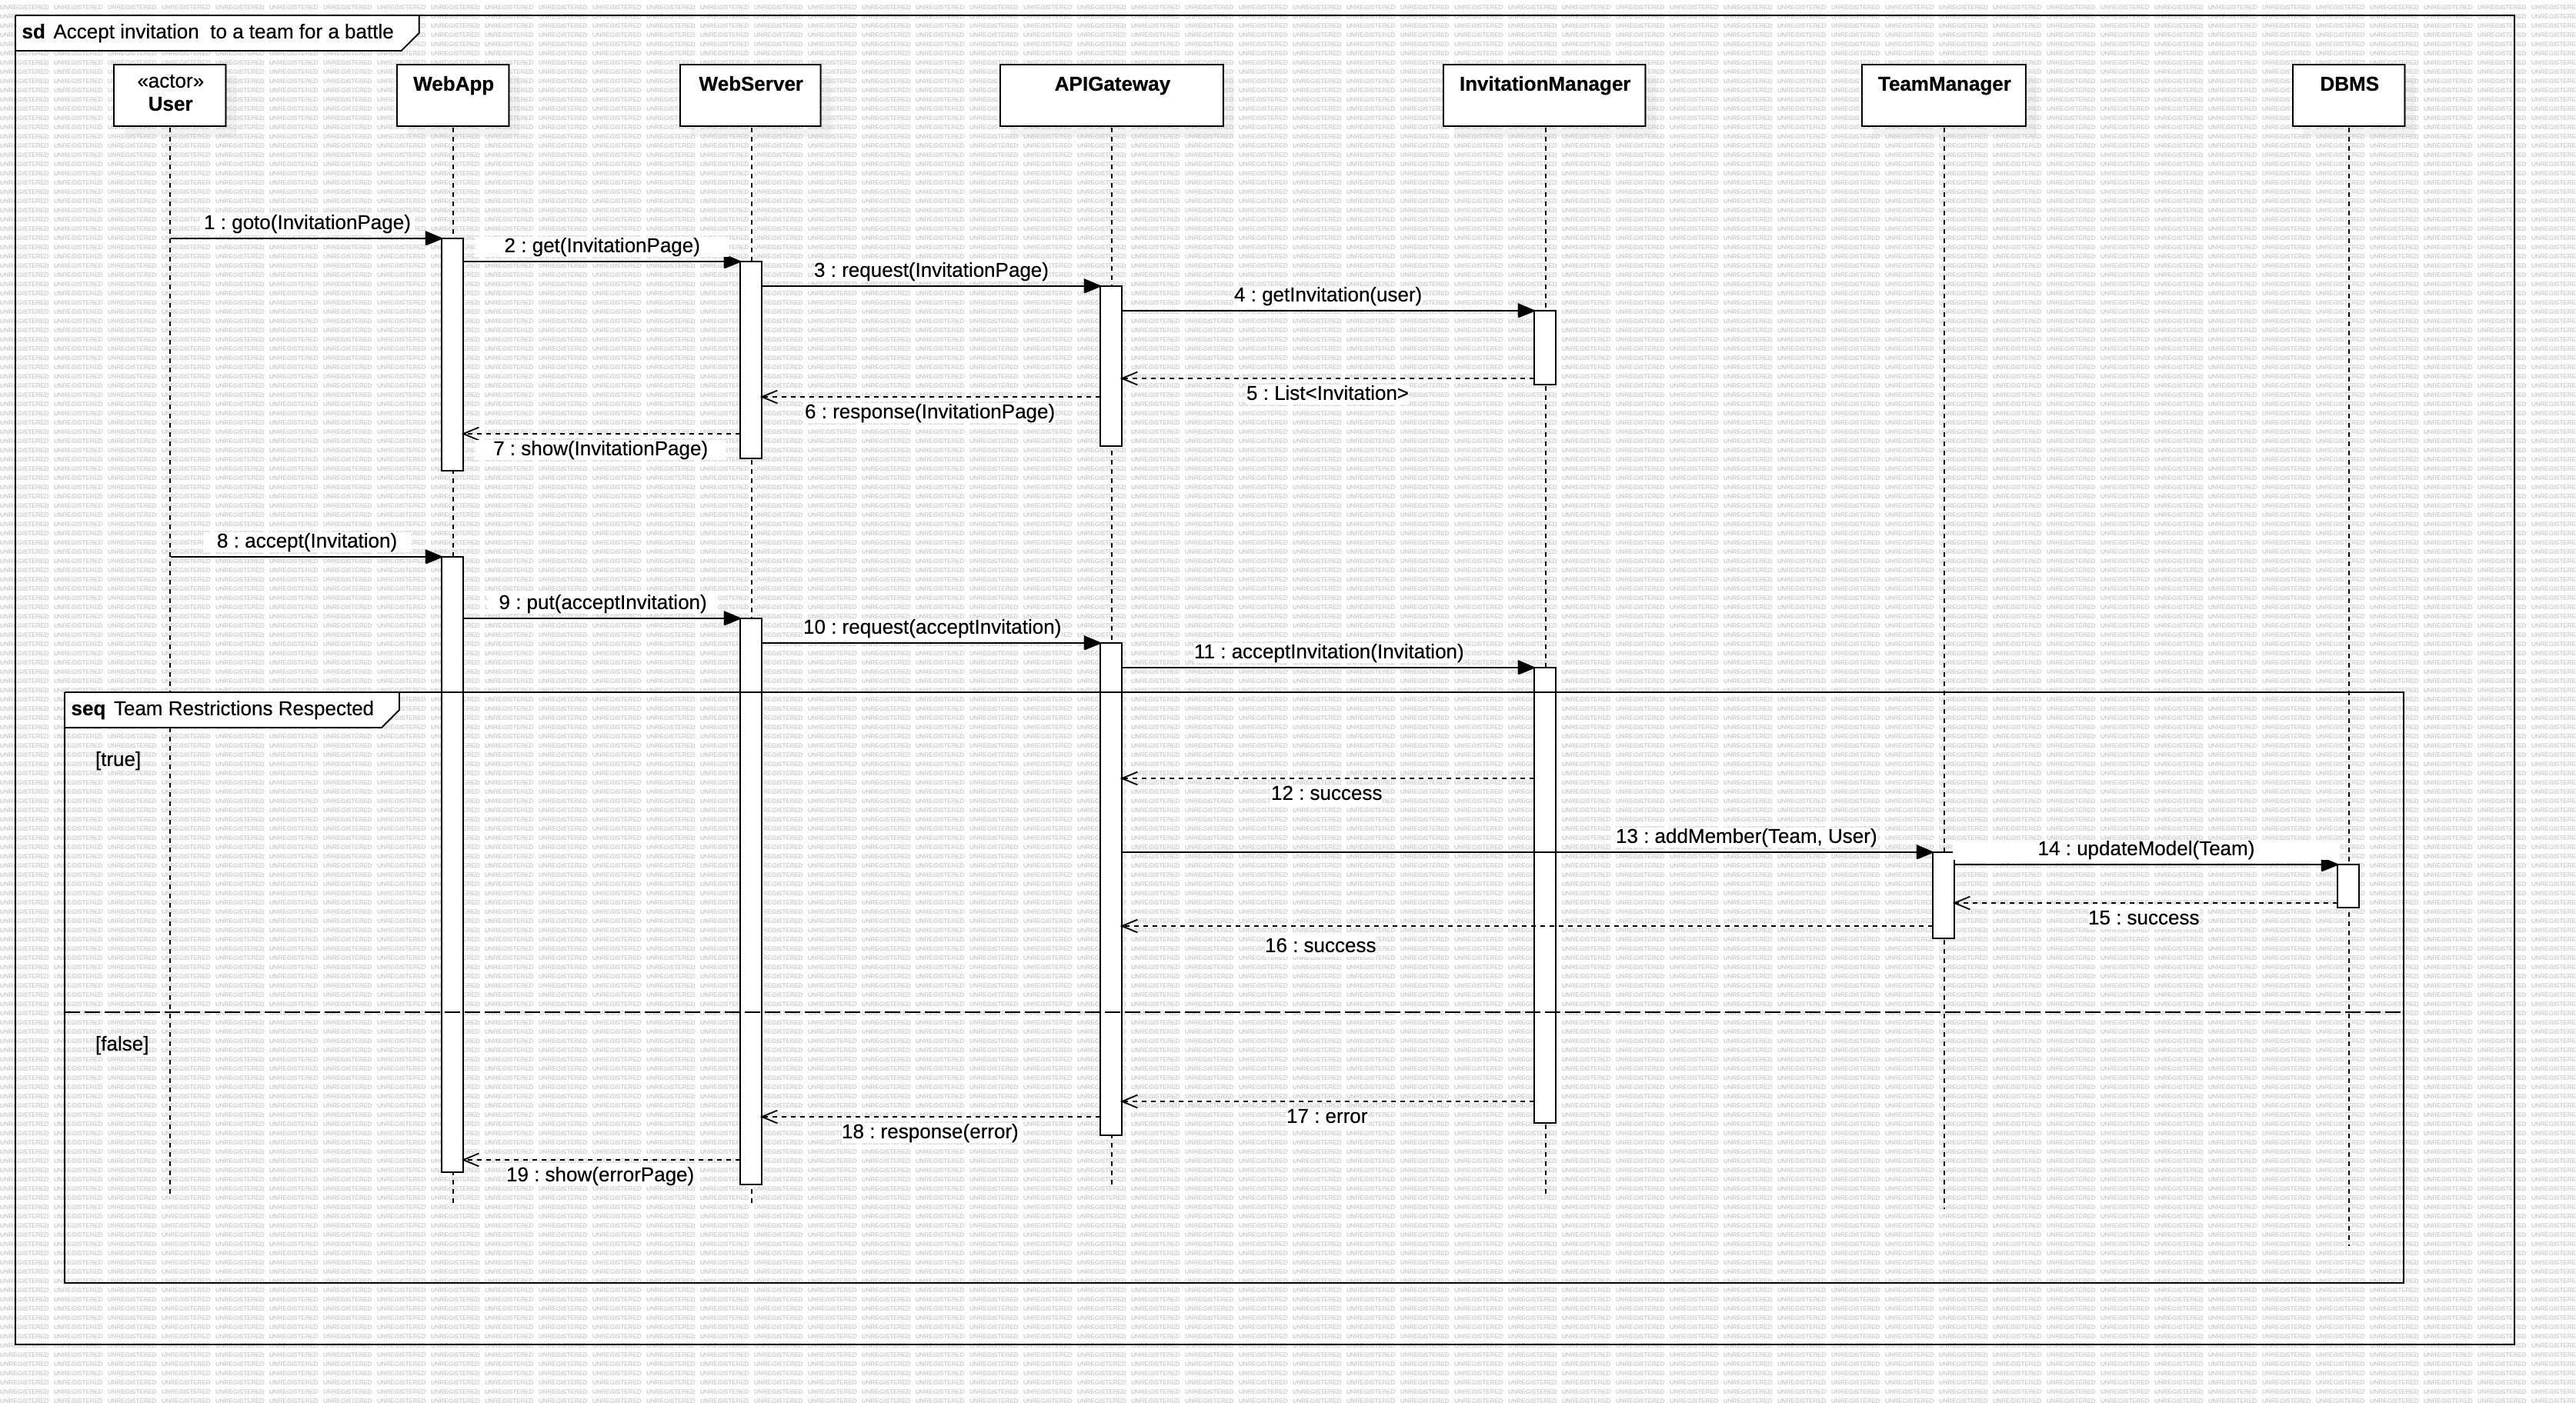
\includegraphics[width=\textwidth]{Diagrams/AcceptInvitationSD.jpg}
    \caption{Runtime view Accept invitation to a team for a battle}
    \label{fig:runtime_view_accept_invitation}
\end{figure}
\subsubsection*{Invite other students to a team}
\begin{figure}[H]
    \centering
    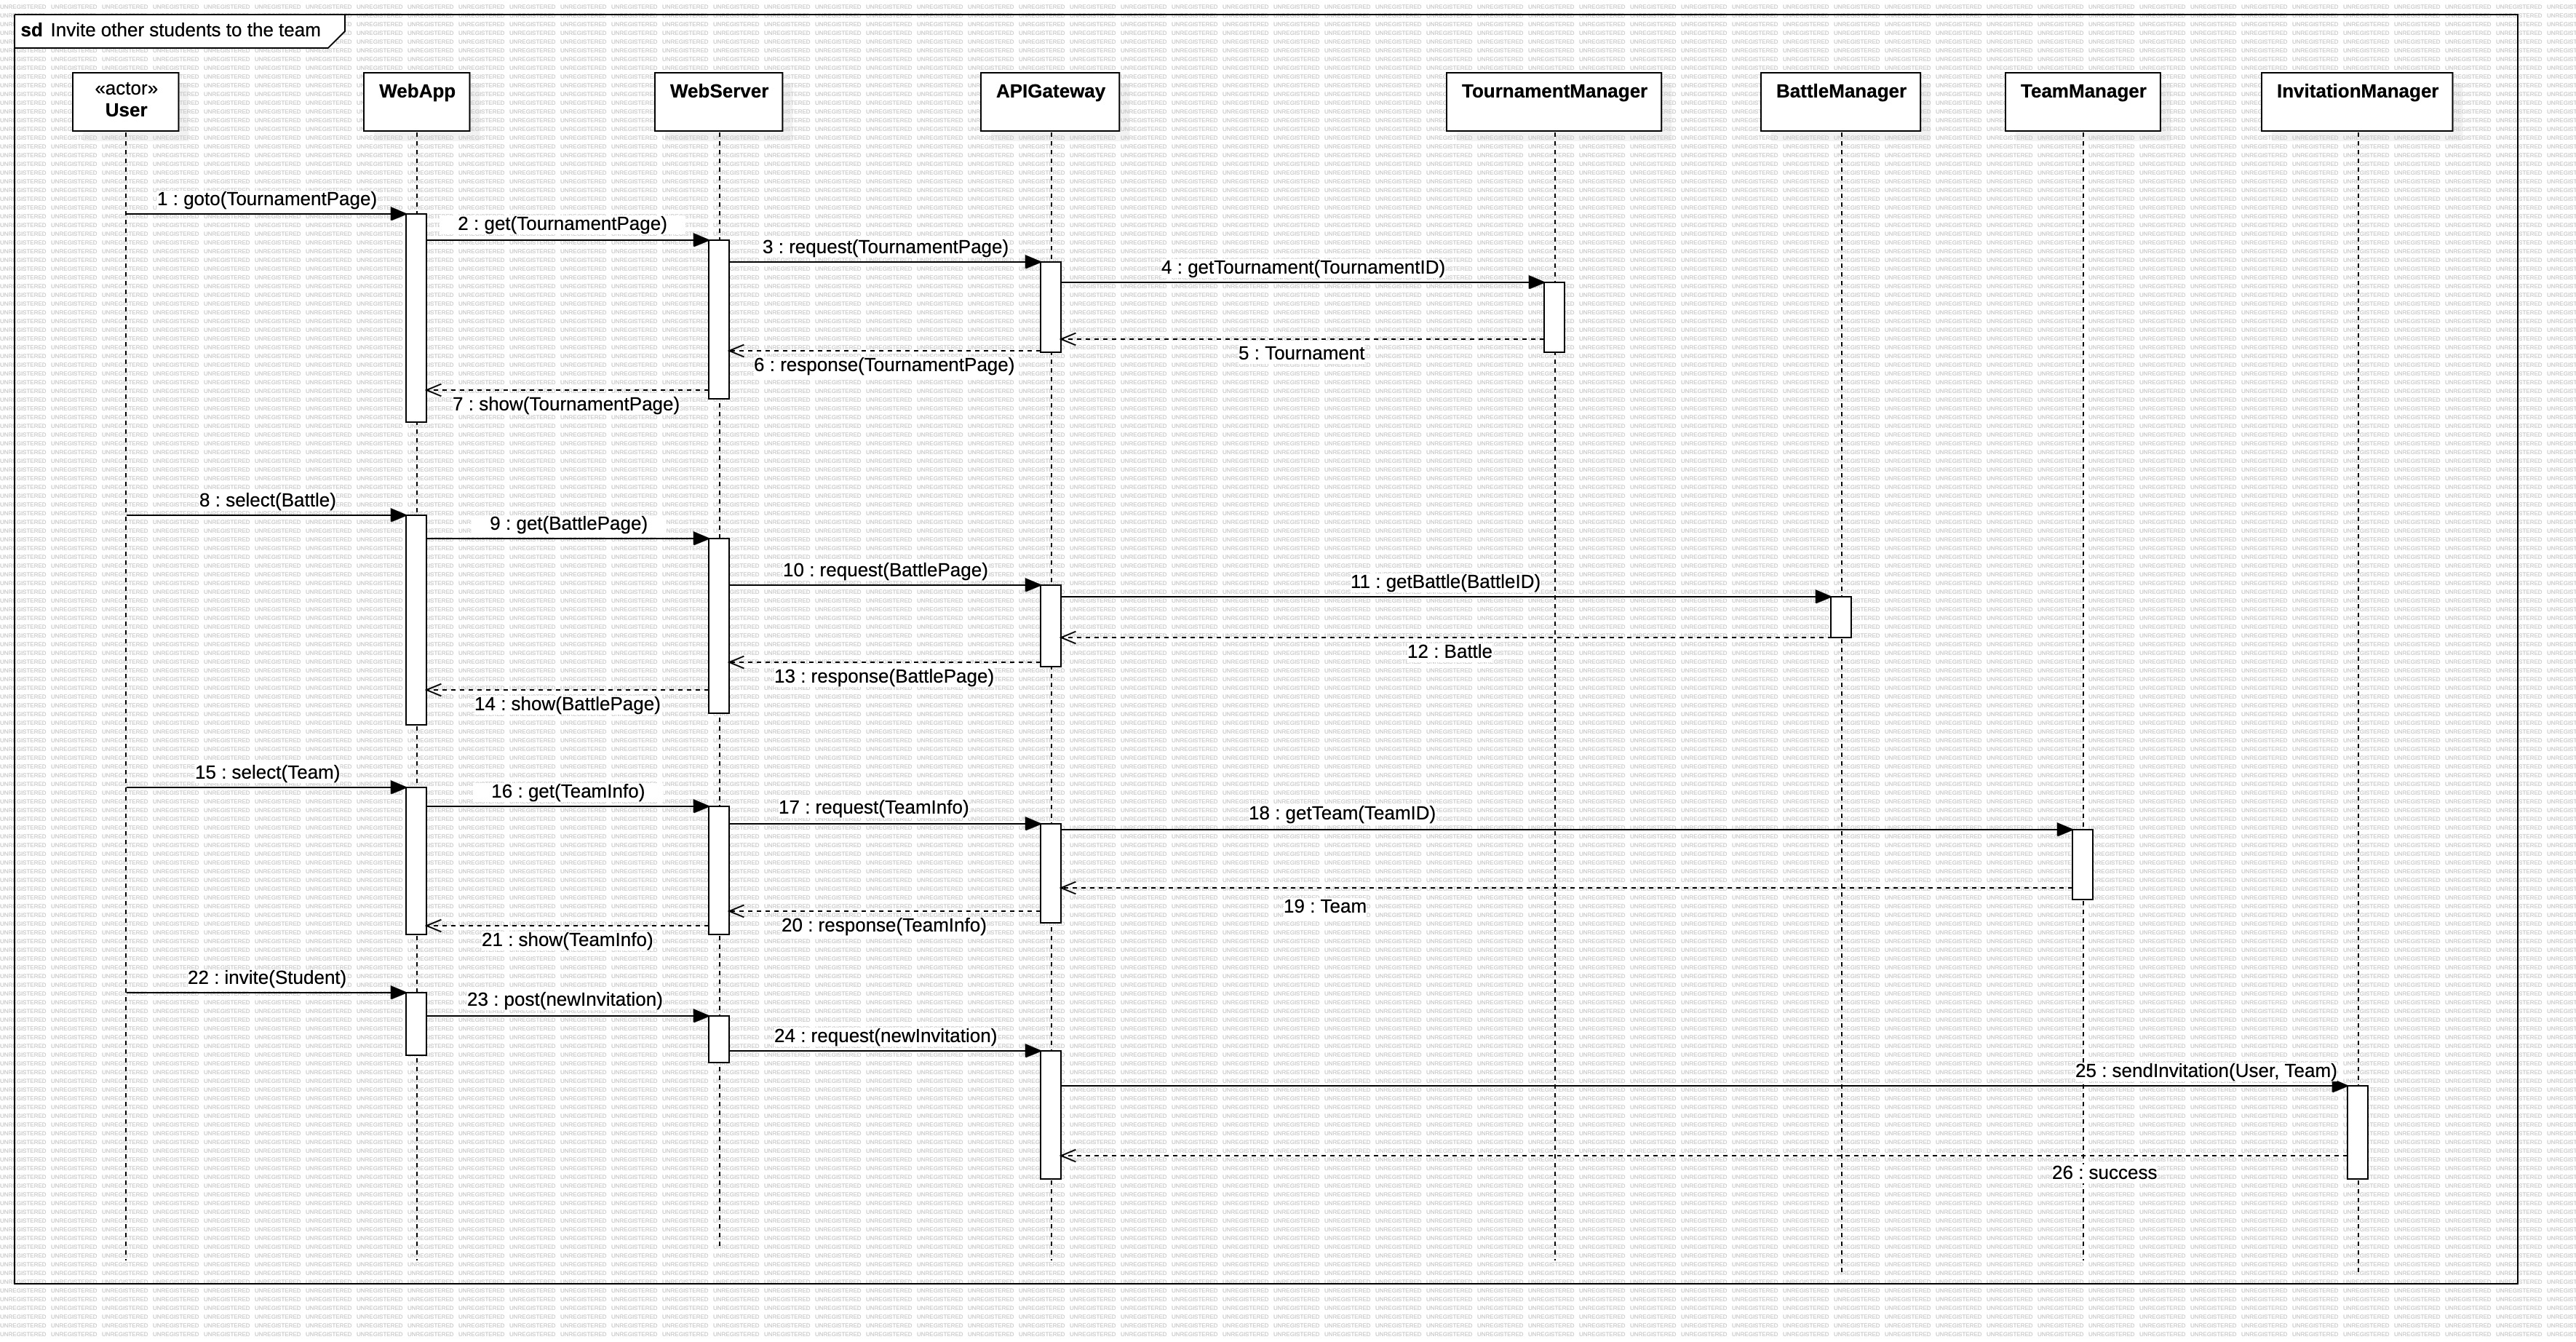
\includegraphics[width=\textwidth]{Diagrams/InviteStudentSD.jpg}
    \caption{Runtime view Invite other students to a team}
    \label{fig:runtime_view_invite_student}
\end{figure}

\subsubsection*{Submission of a solution and Automatic evaluation}
\begin{figure}[H]
    \centering
    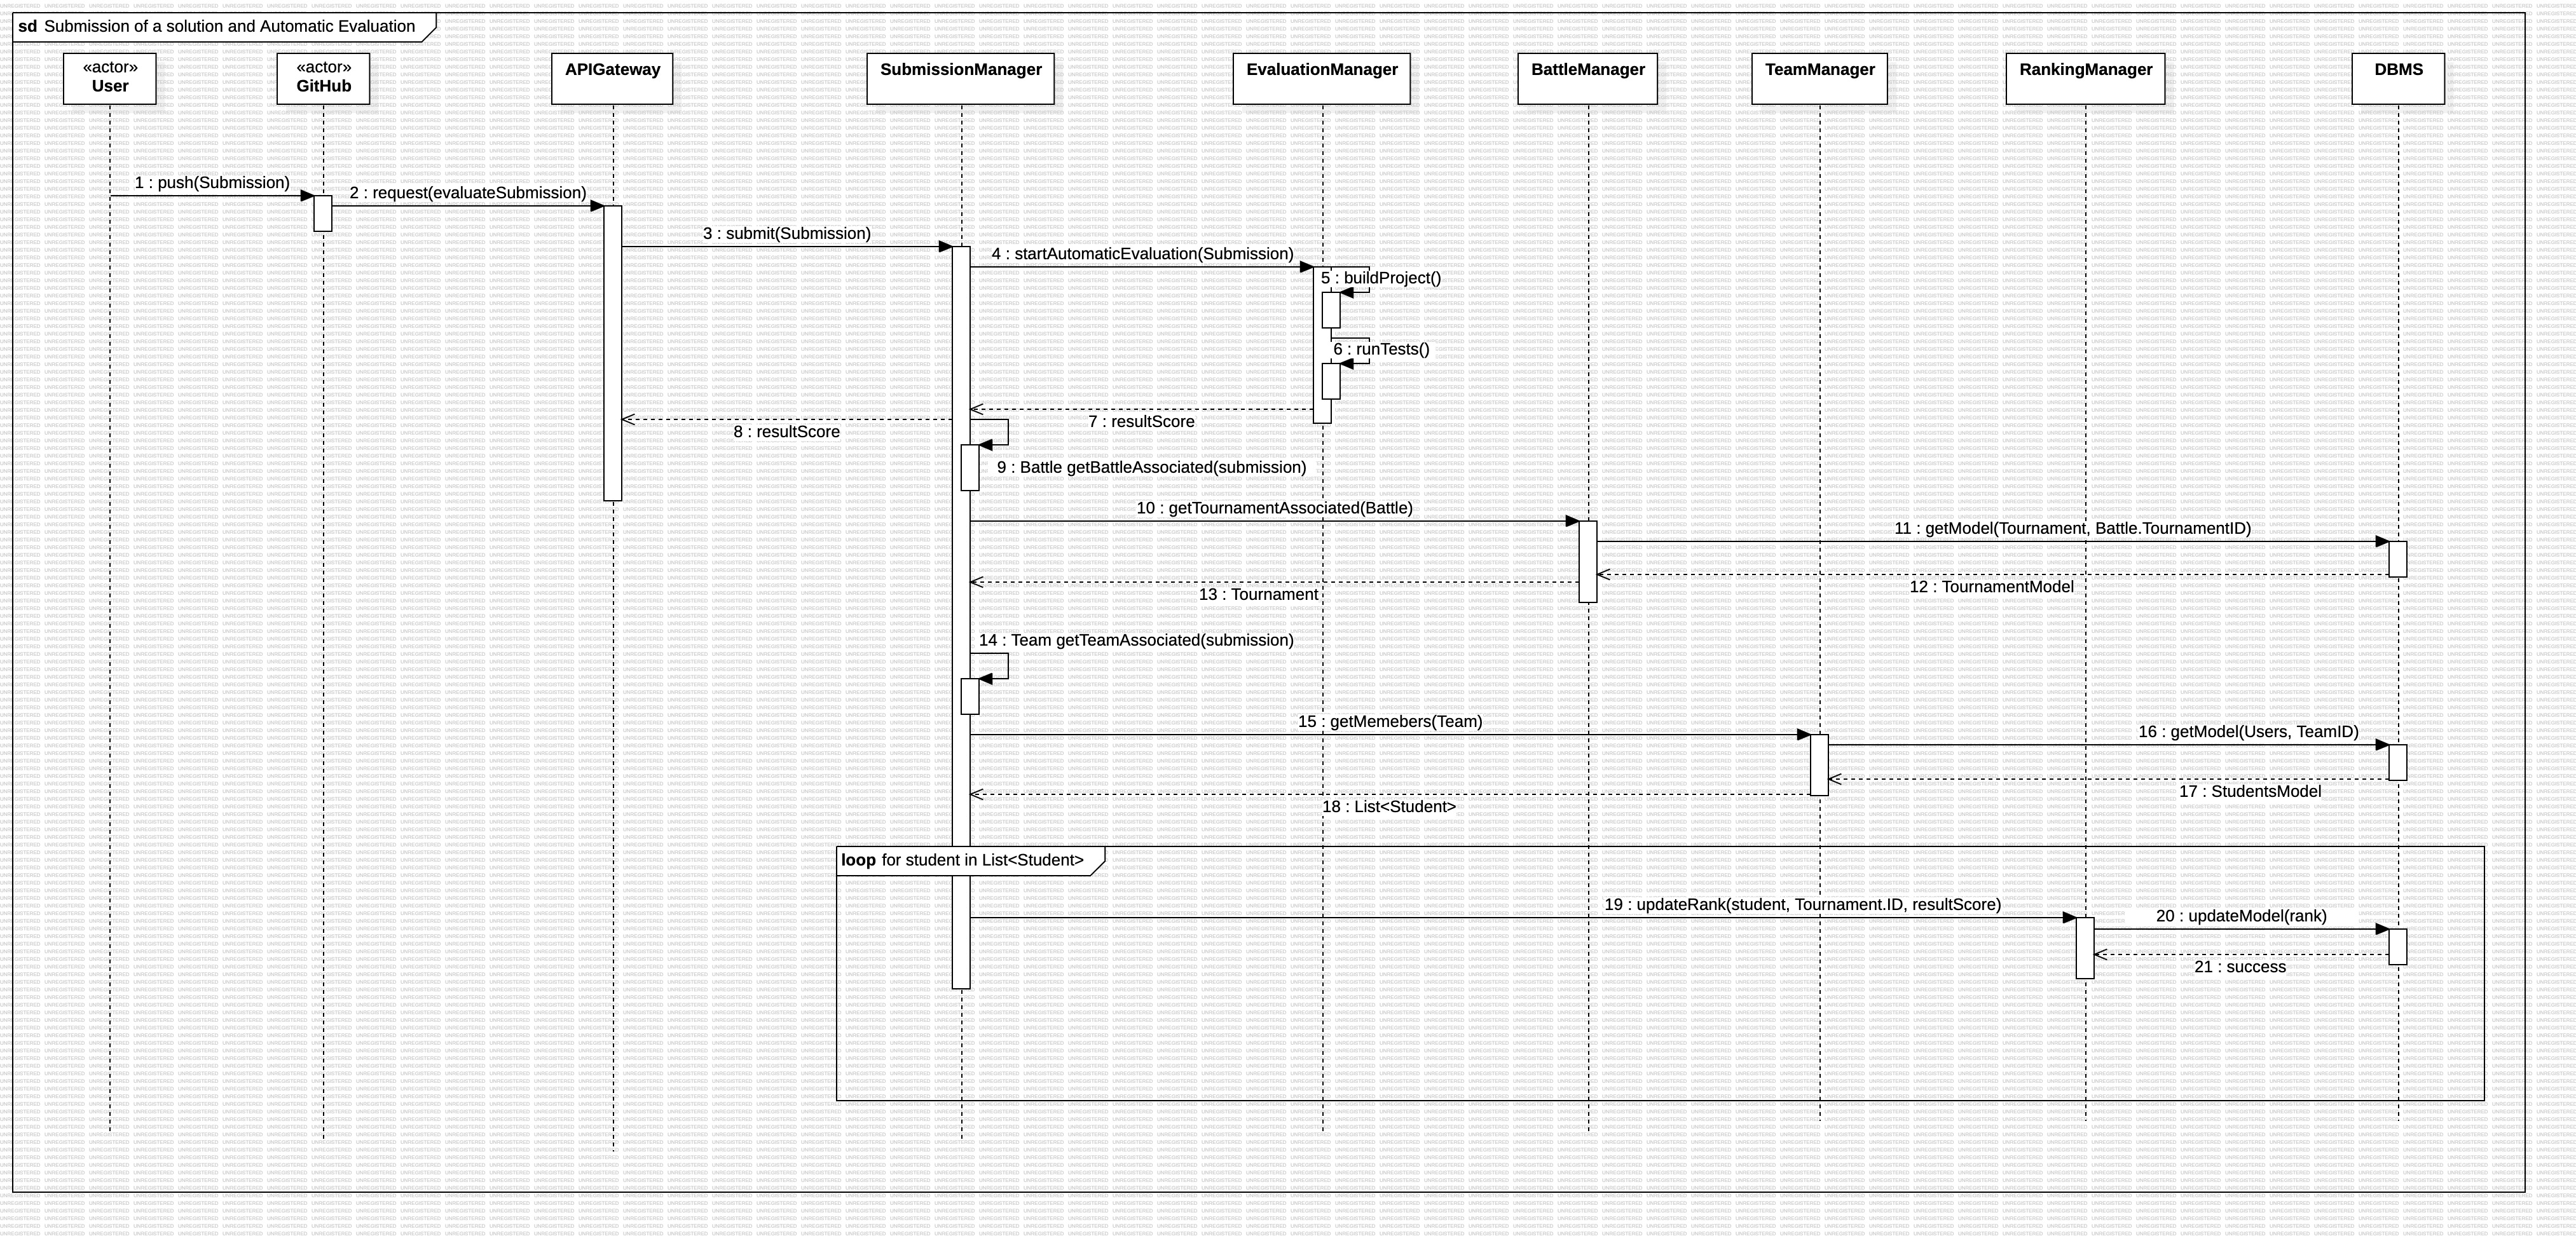
\includegraphics[width=\textwidth]{Diagrams/SolutionSubmissionSD.jpg}
    \caption{Runtime view Submit a solution and Automatic evaluation}
    \label{fig:runtime_view_submit_solution}
\end{figure}

\subsubsection*{Close a Tournament}
\begin{figure}[H]
    \centering
    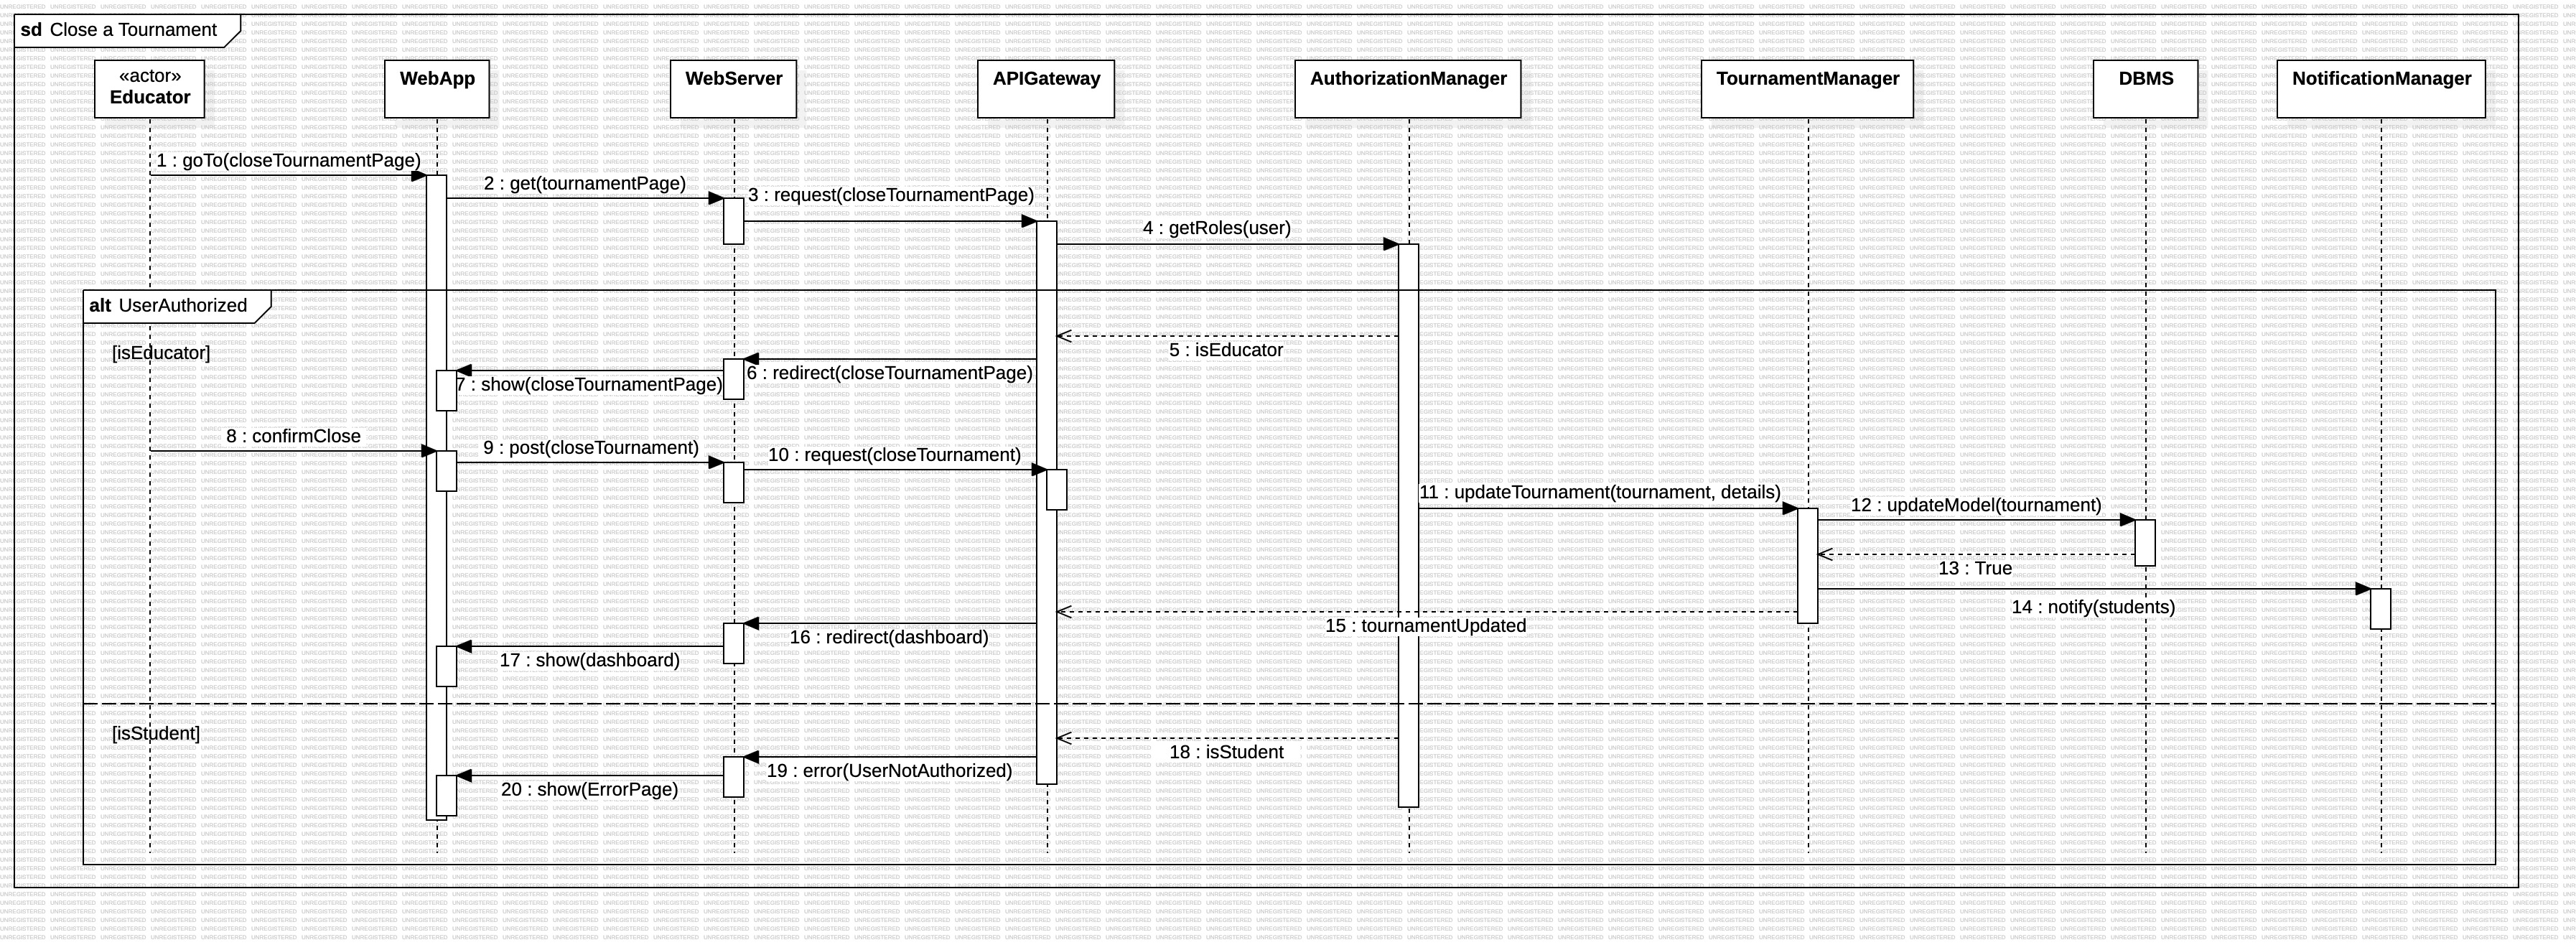
\includegraphics[width=\textwidth]{Diagrams/CloseTournamentSD.jpg}
    \caption{Runtime view}
    \label{fig:runtime_view}
\end{figure}

\subsubsection*{Upload of CodeKata}
\begin{figure}[H]
    \centering
    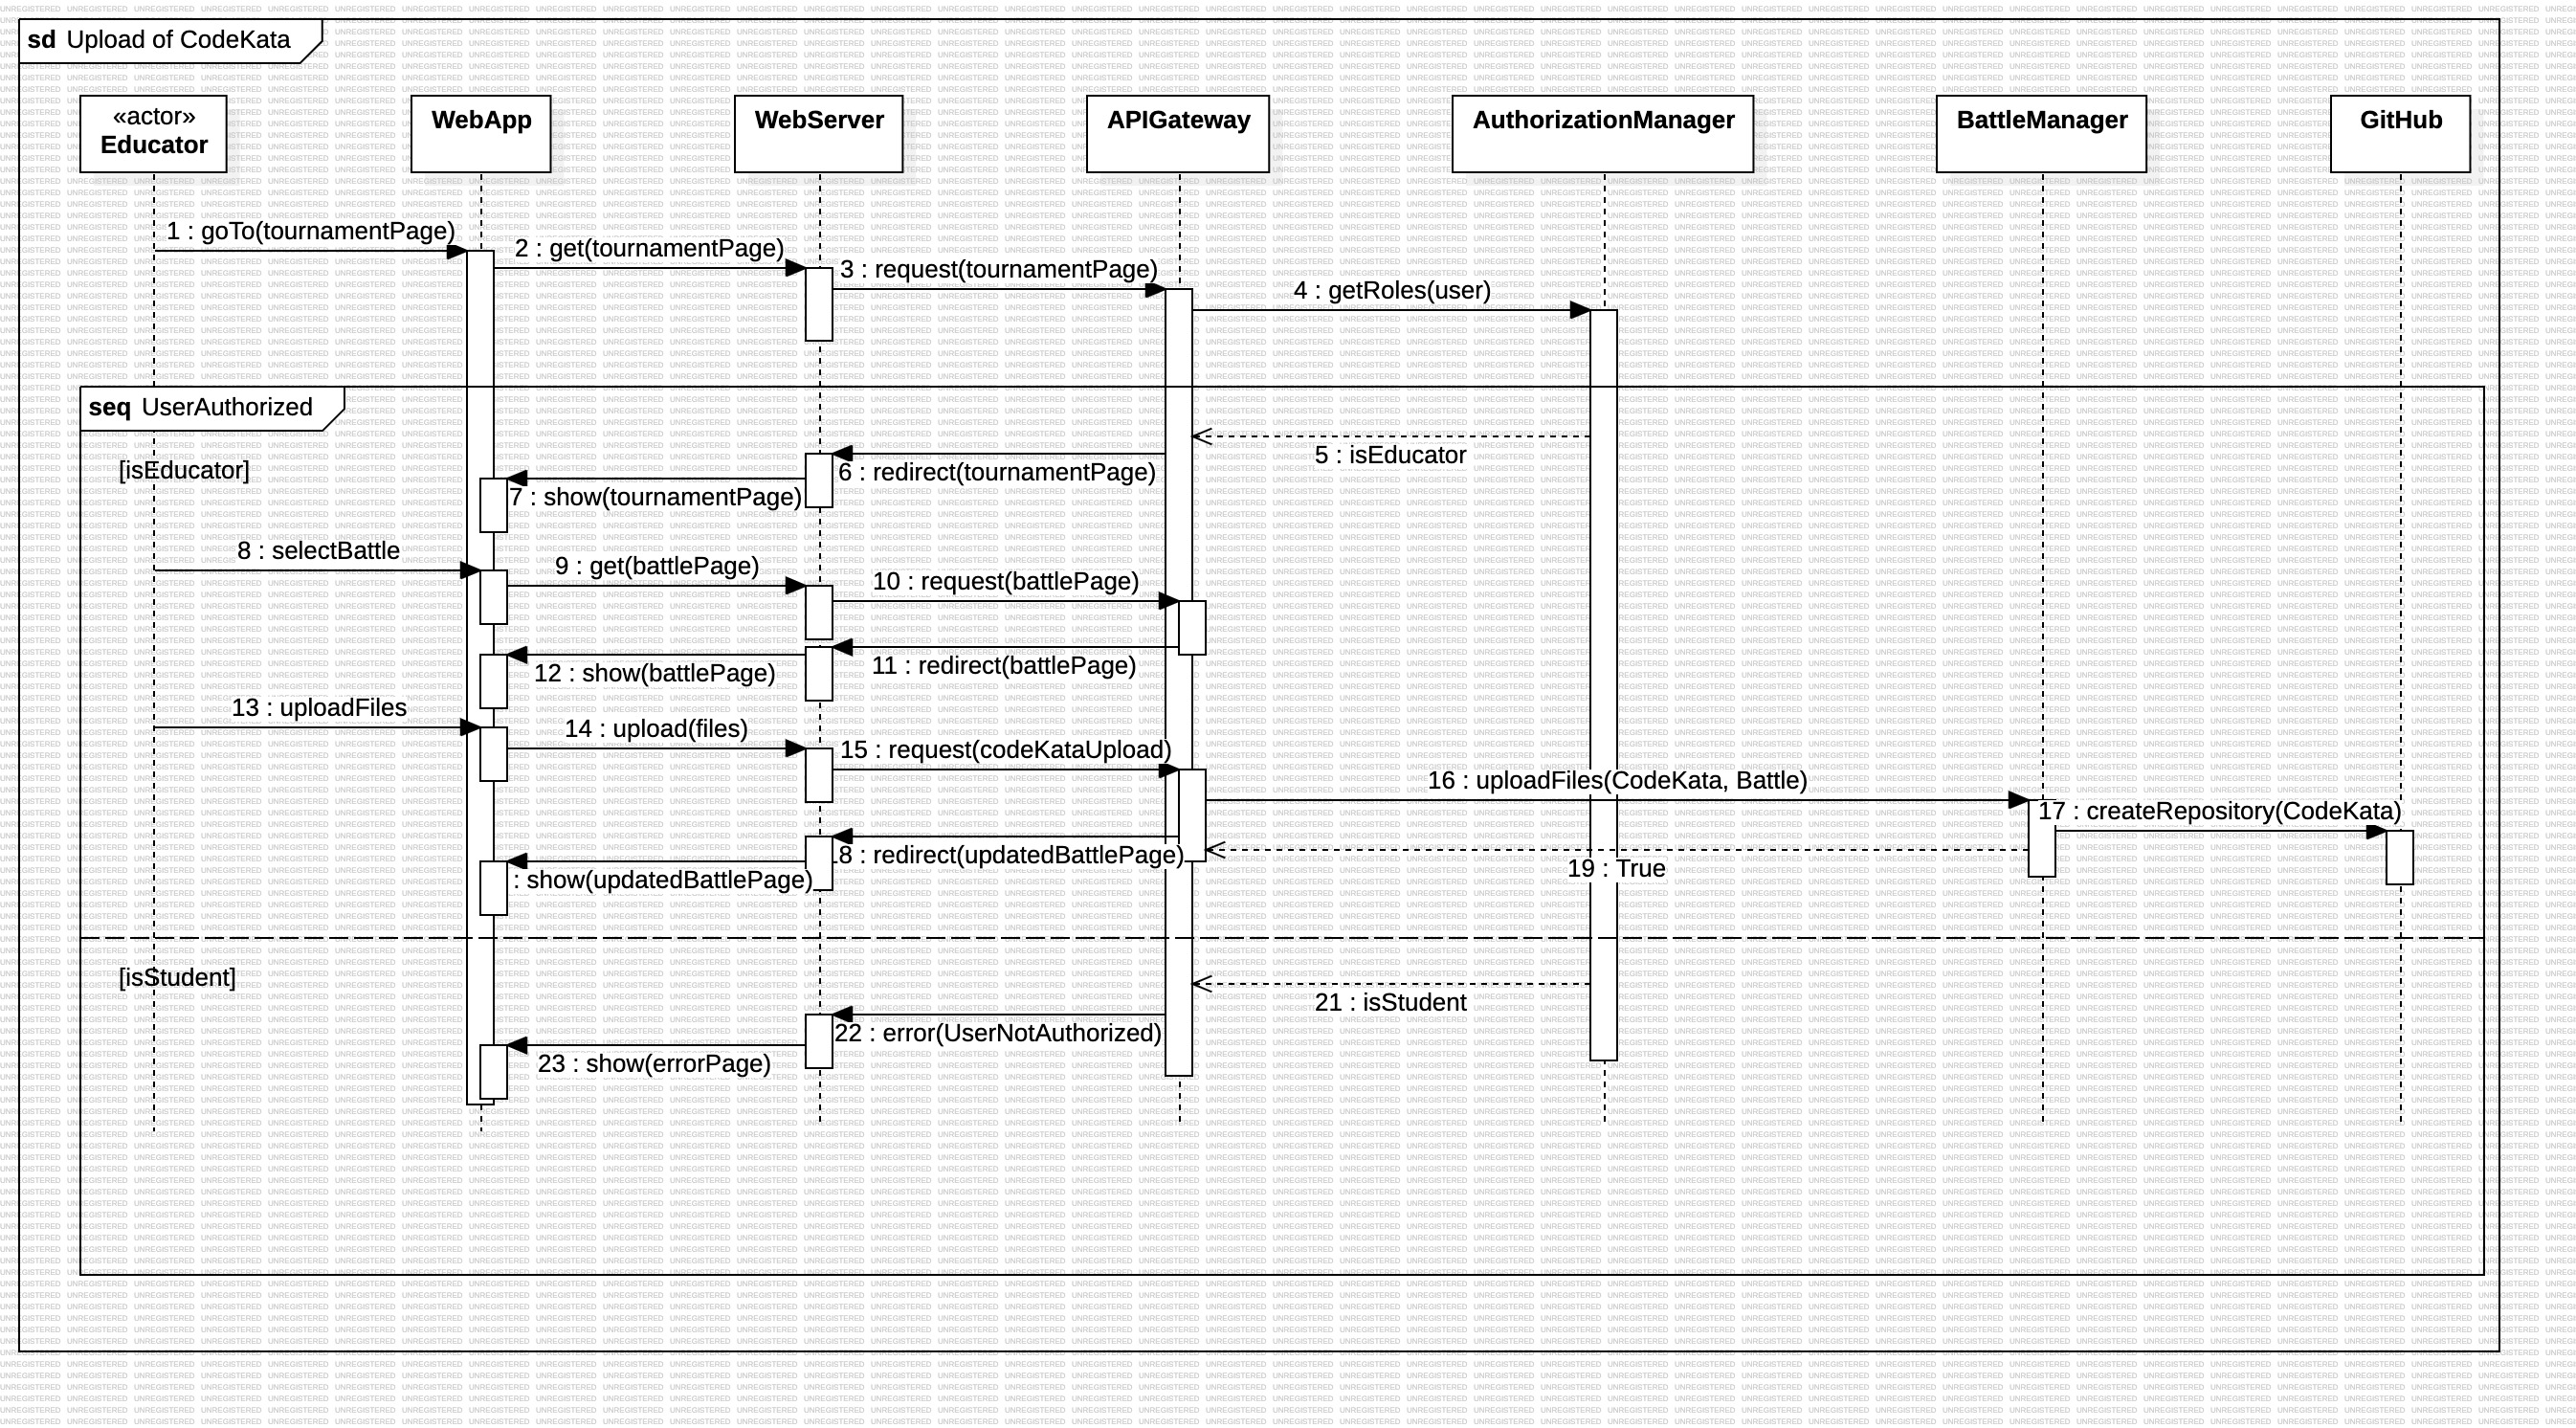
\includegraphics[width=\textwidth]{Diagrams/UploadCodeKataSD.jpg}
    \caption{Runtime view}
    \label{fig:runtime_view}
\end{figure}

\subsubsection*{Manual Score Update}
\begin{figure}[H]
    \centering
    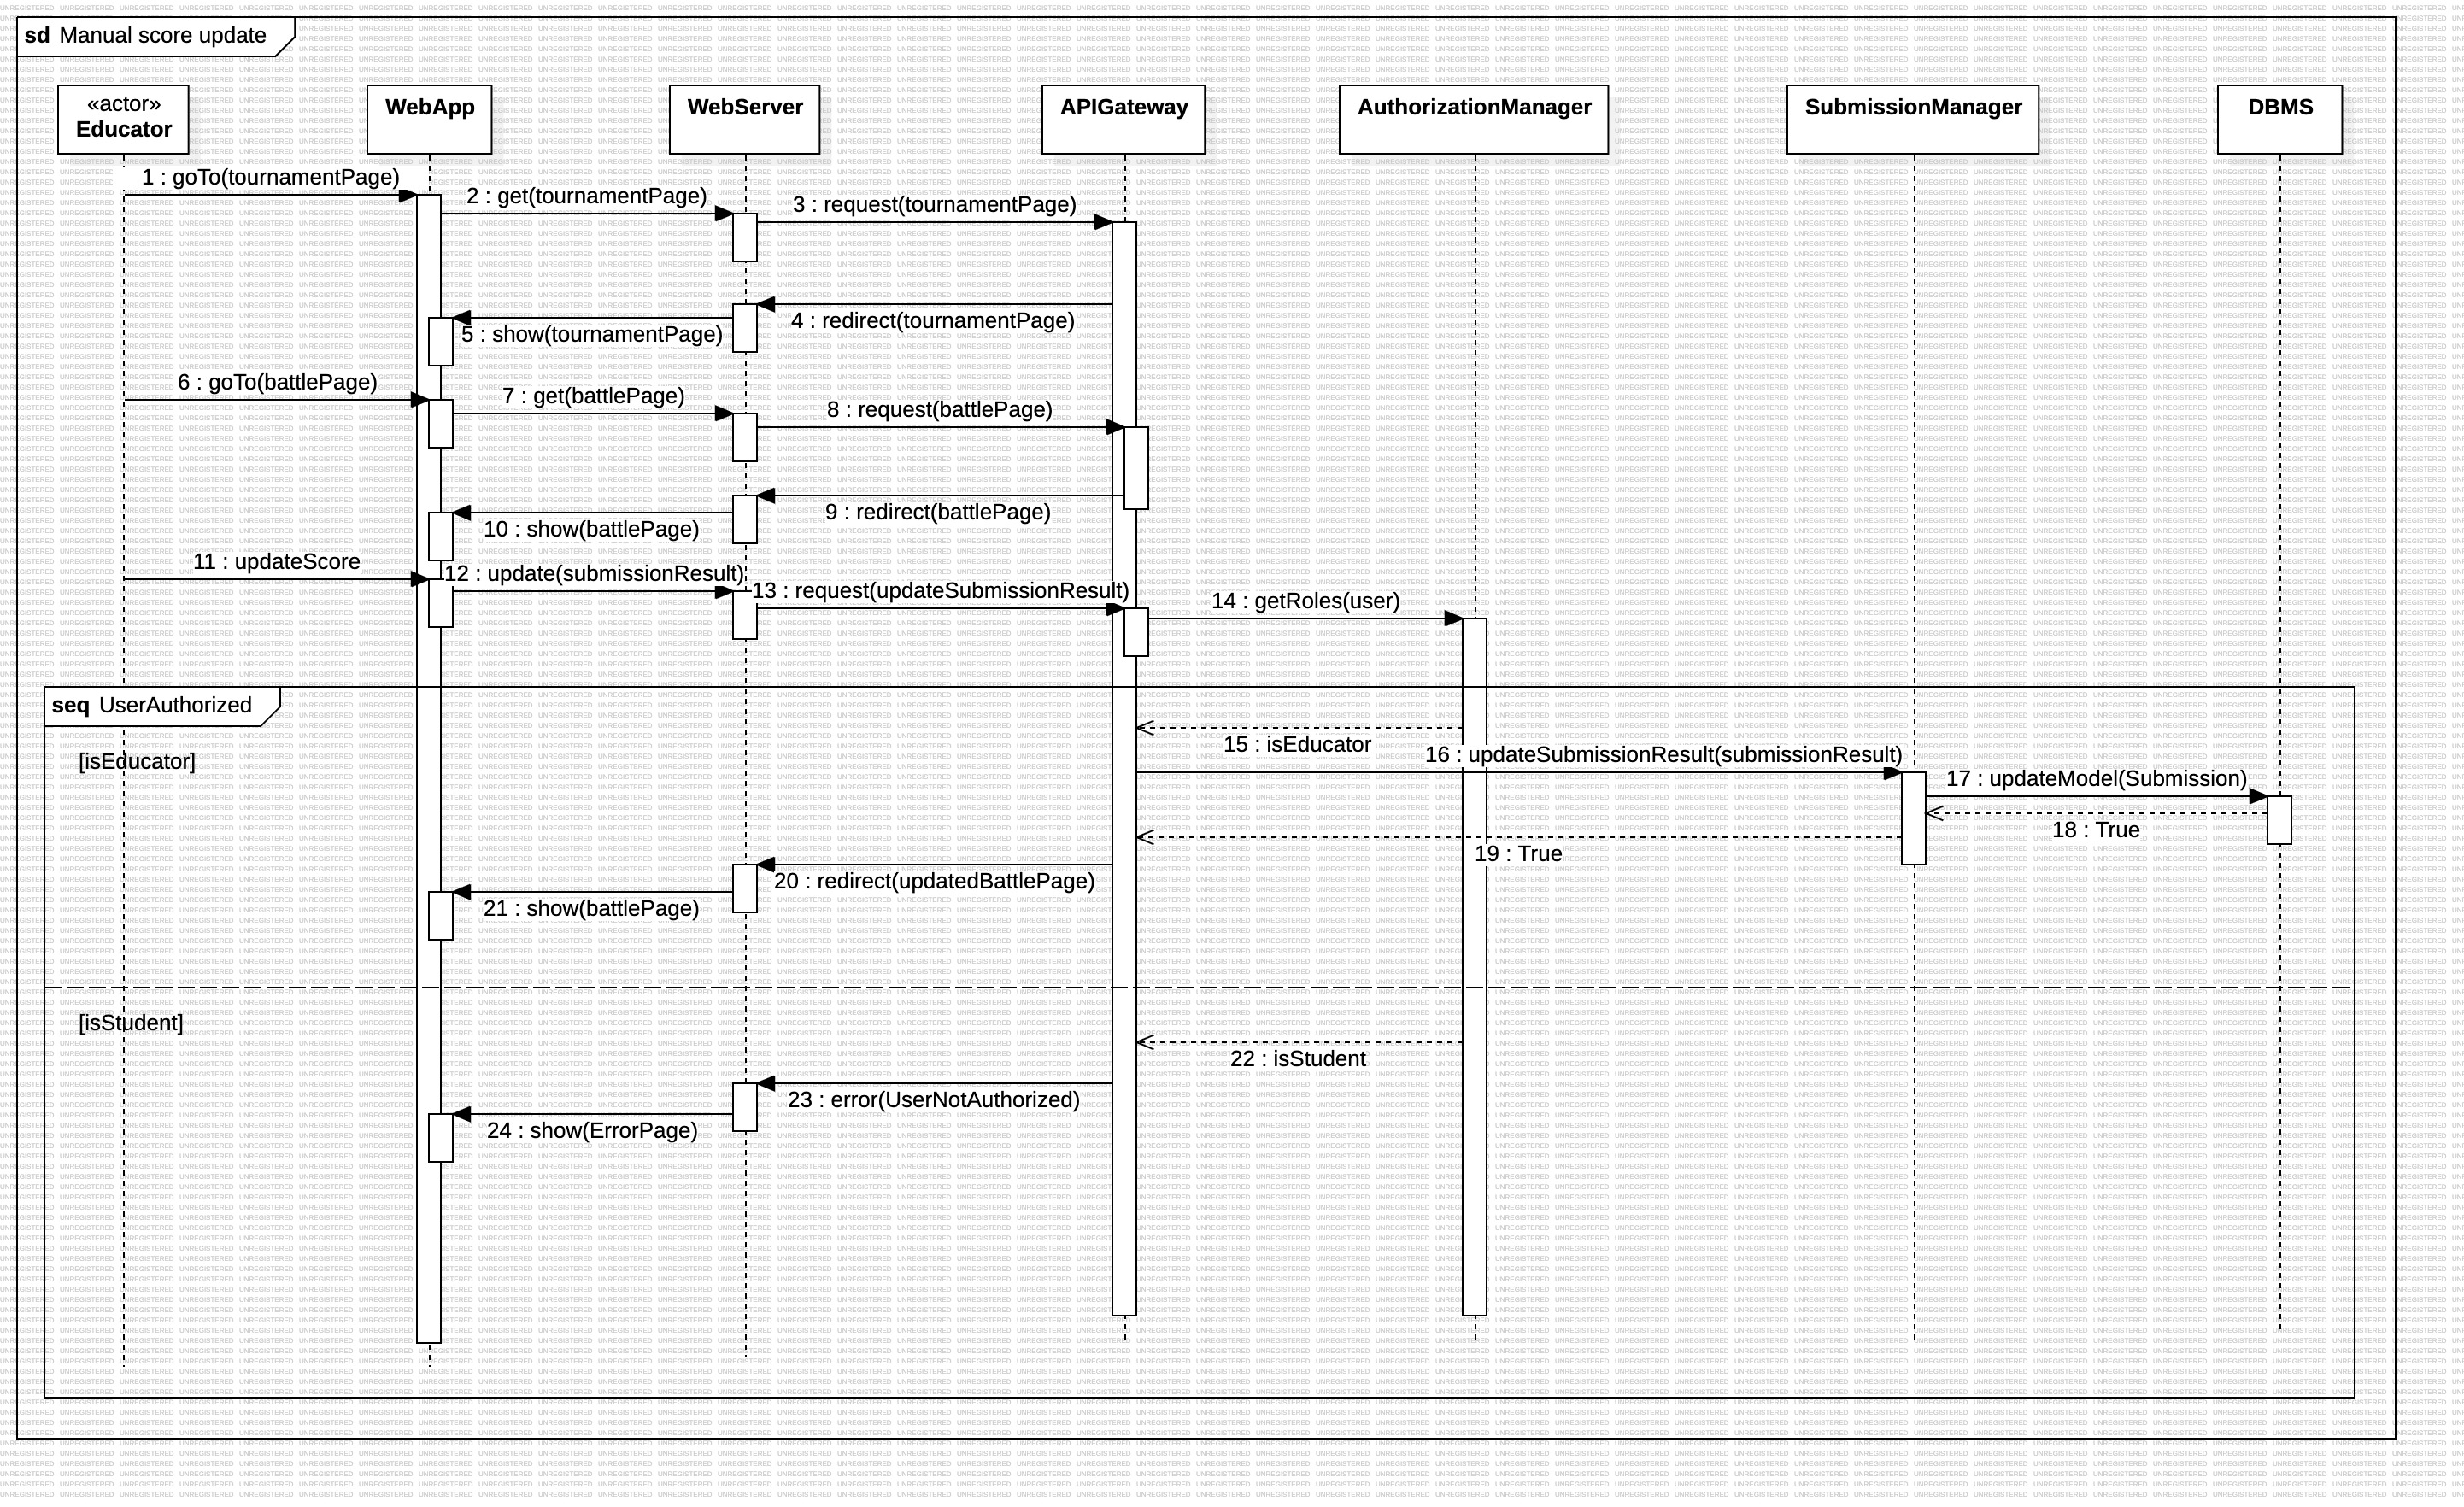
\includegraphics[width=\textwidth]{Diagrams/ManualScoreUpdateSD.jpg}
    \caption{Runtime view}
    \label{fig:runtime_view}
\end{figure}

\subsubsection*{Notification to a Student}
\begin{figure}[H]
    \centering
    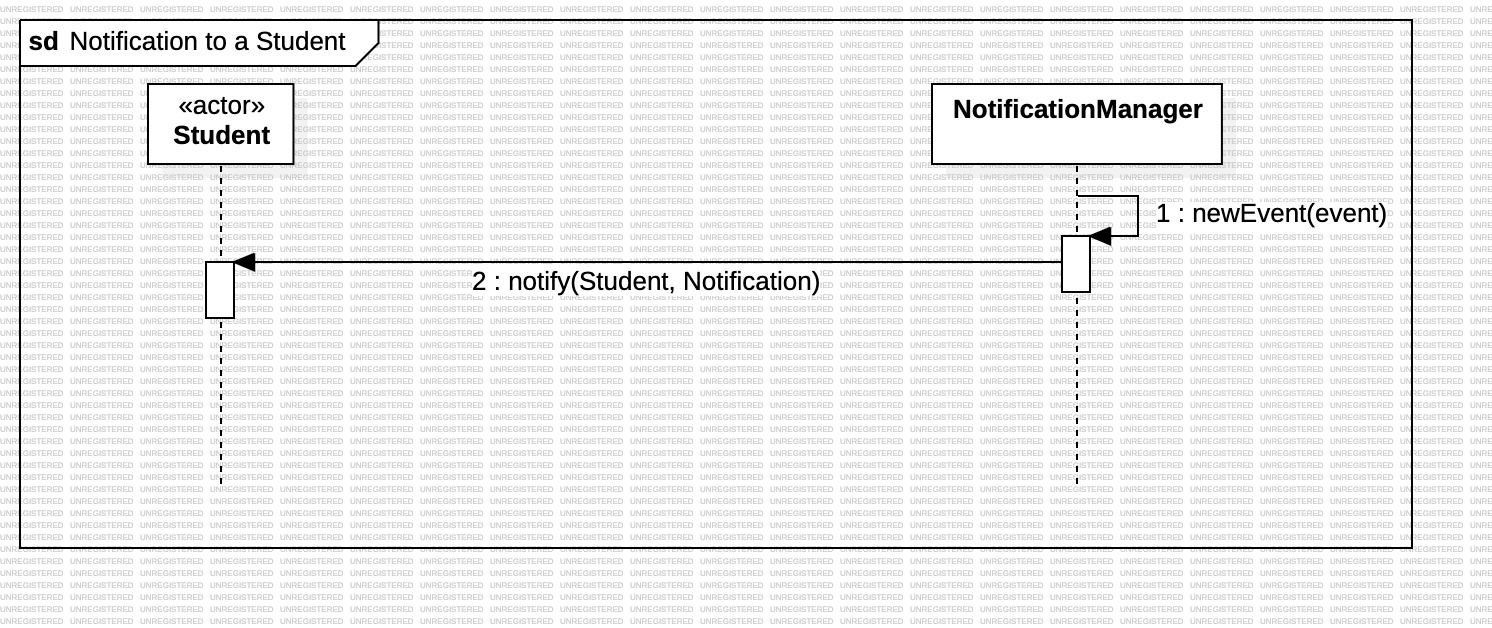
\includegraphics[width=\textwidth]{Diagrams/NotificationToStudentSD.jpg}
    \caption{Runtime view}
    \label{fig:runtime_view}
\end{figure}

\subsubsection*{Subscribe to a Battle}
\begin{figure}[H]
    \centering
    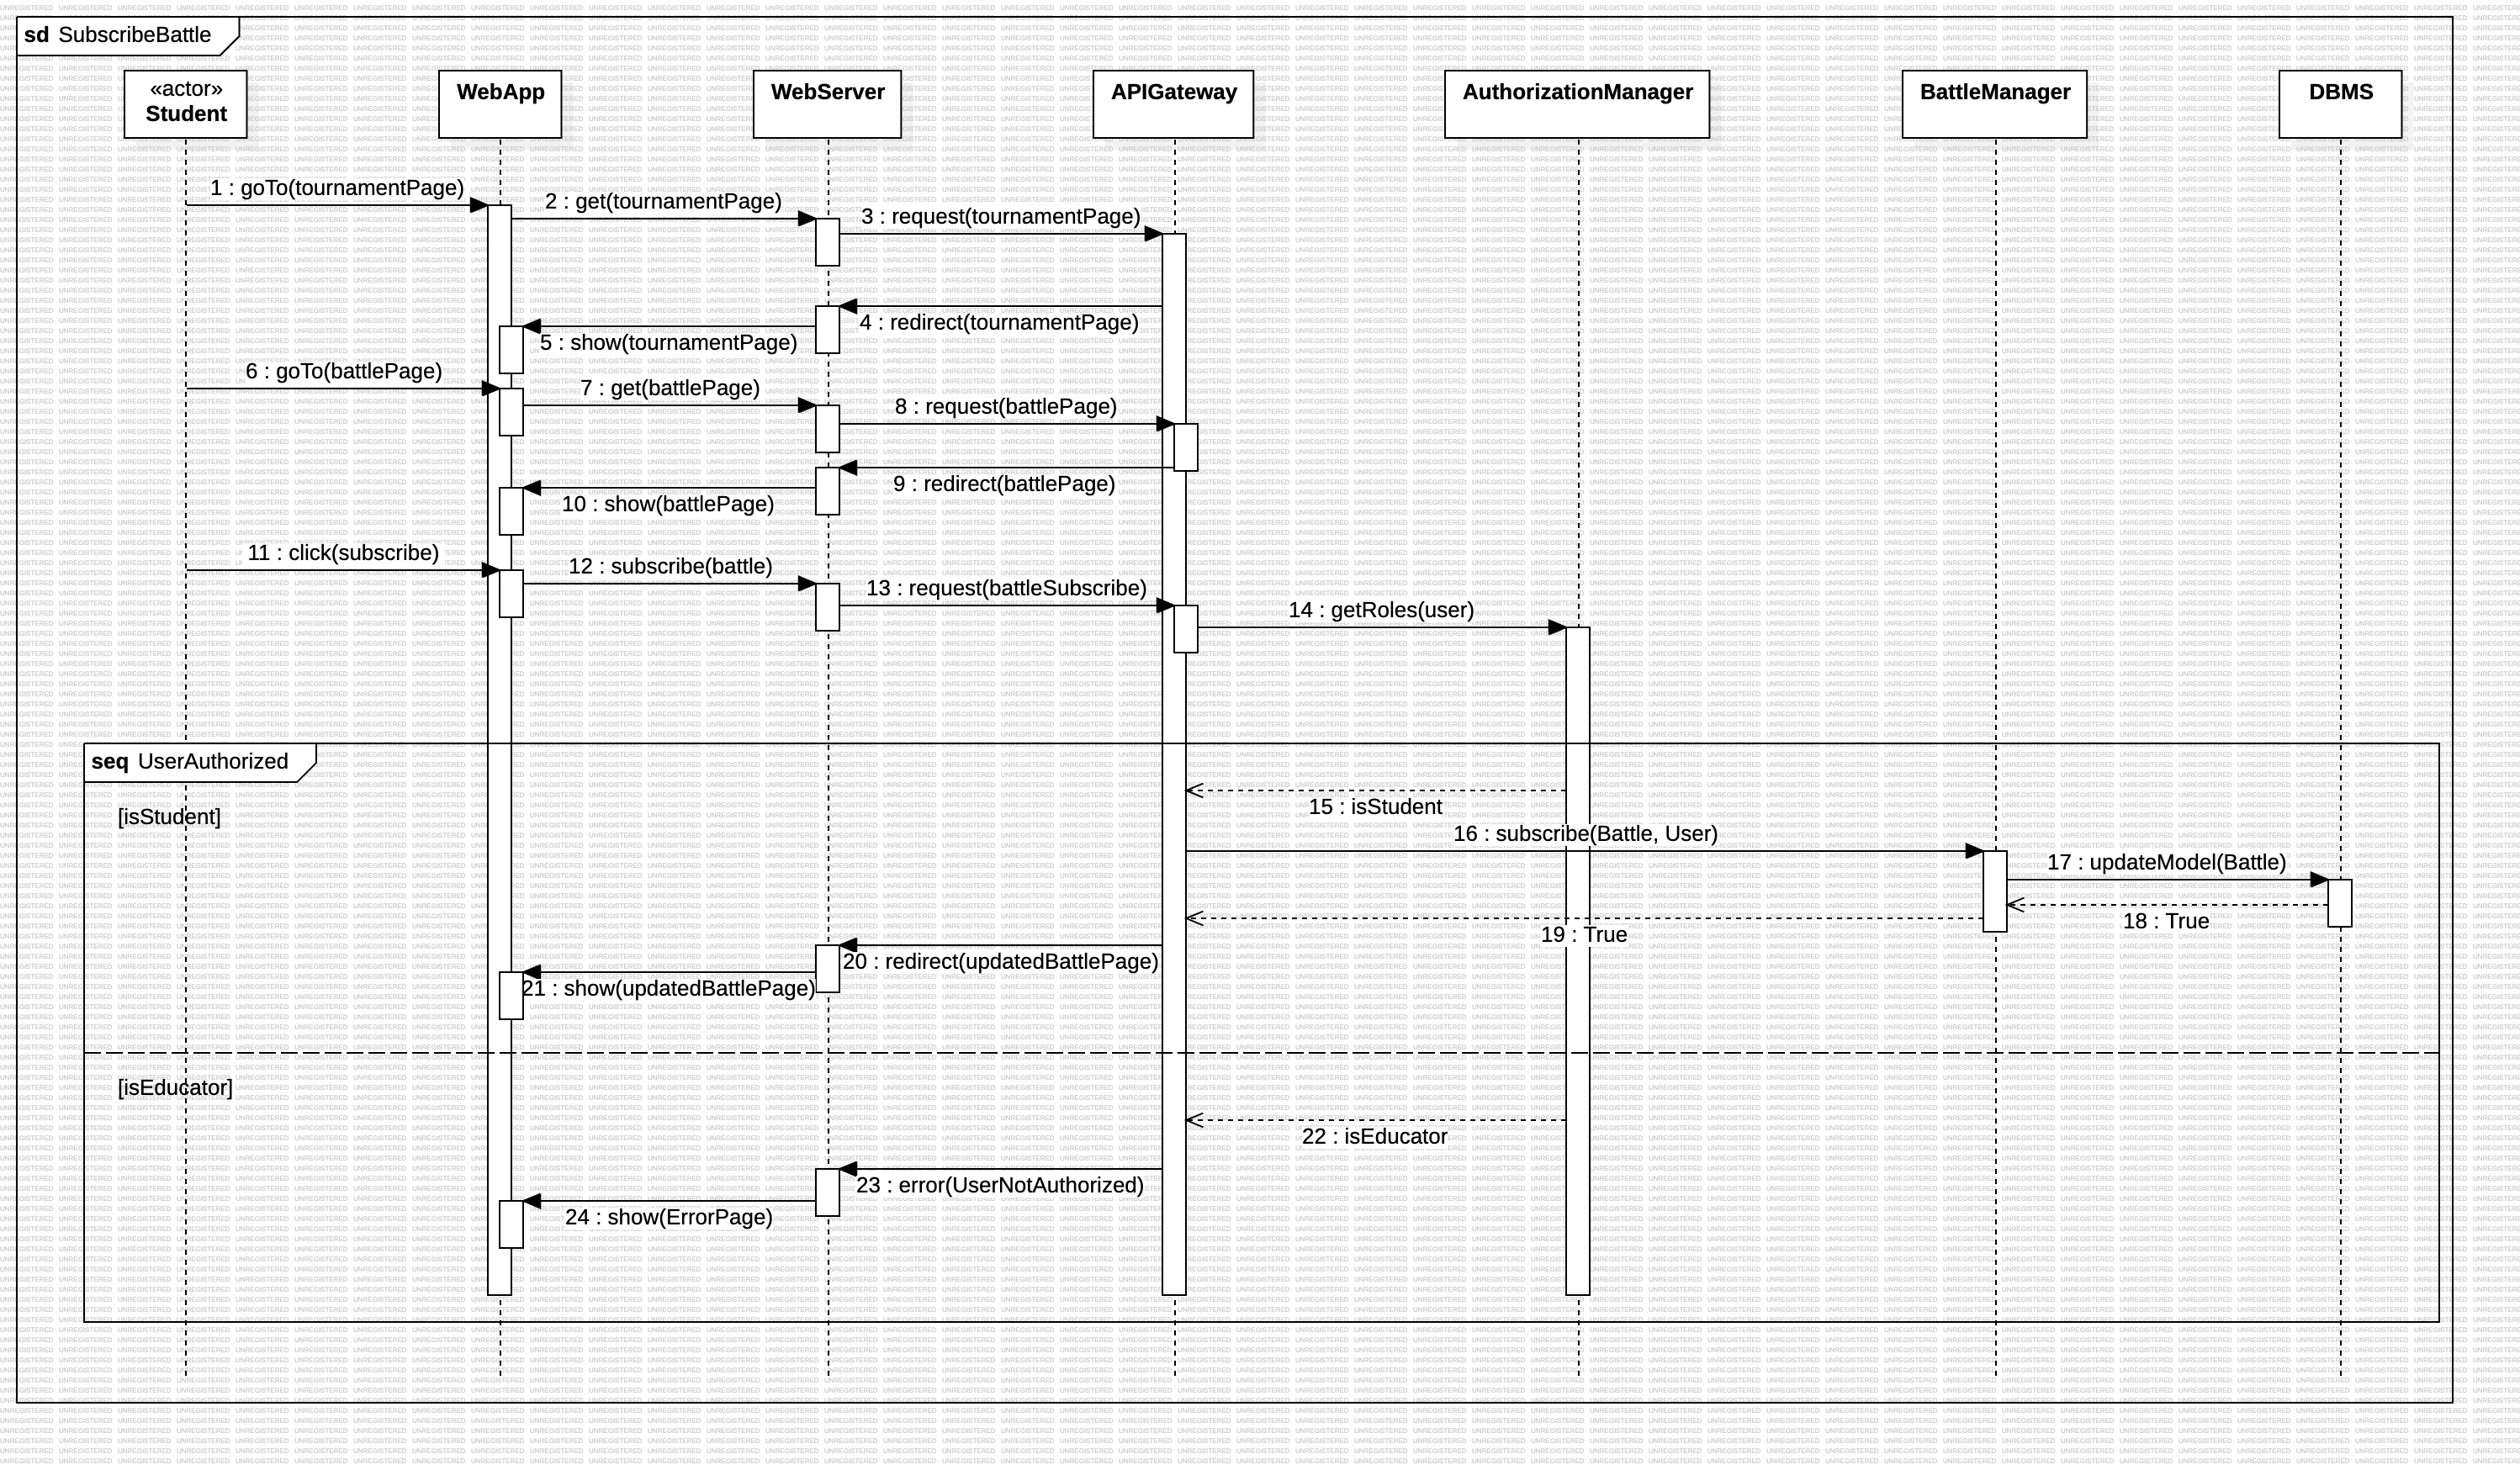
\includegraphics[width=\textwidth]{Diagrams/SubscribeBattleSD.jpg}
    \caption{Runtime view}
\label{fig:runtime_view}
\end{figure}

\subsubsection*{Fork repository of a Battle}
\begin{figure}[H]
    \centering
    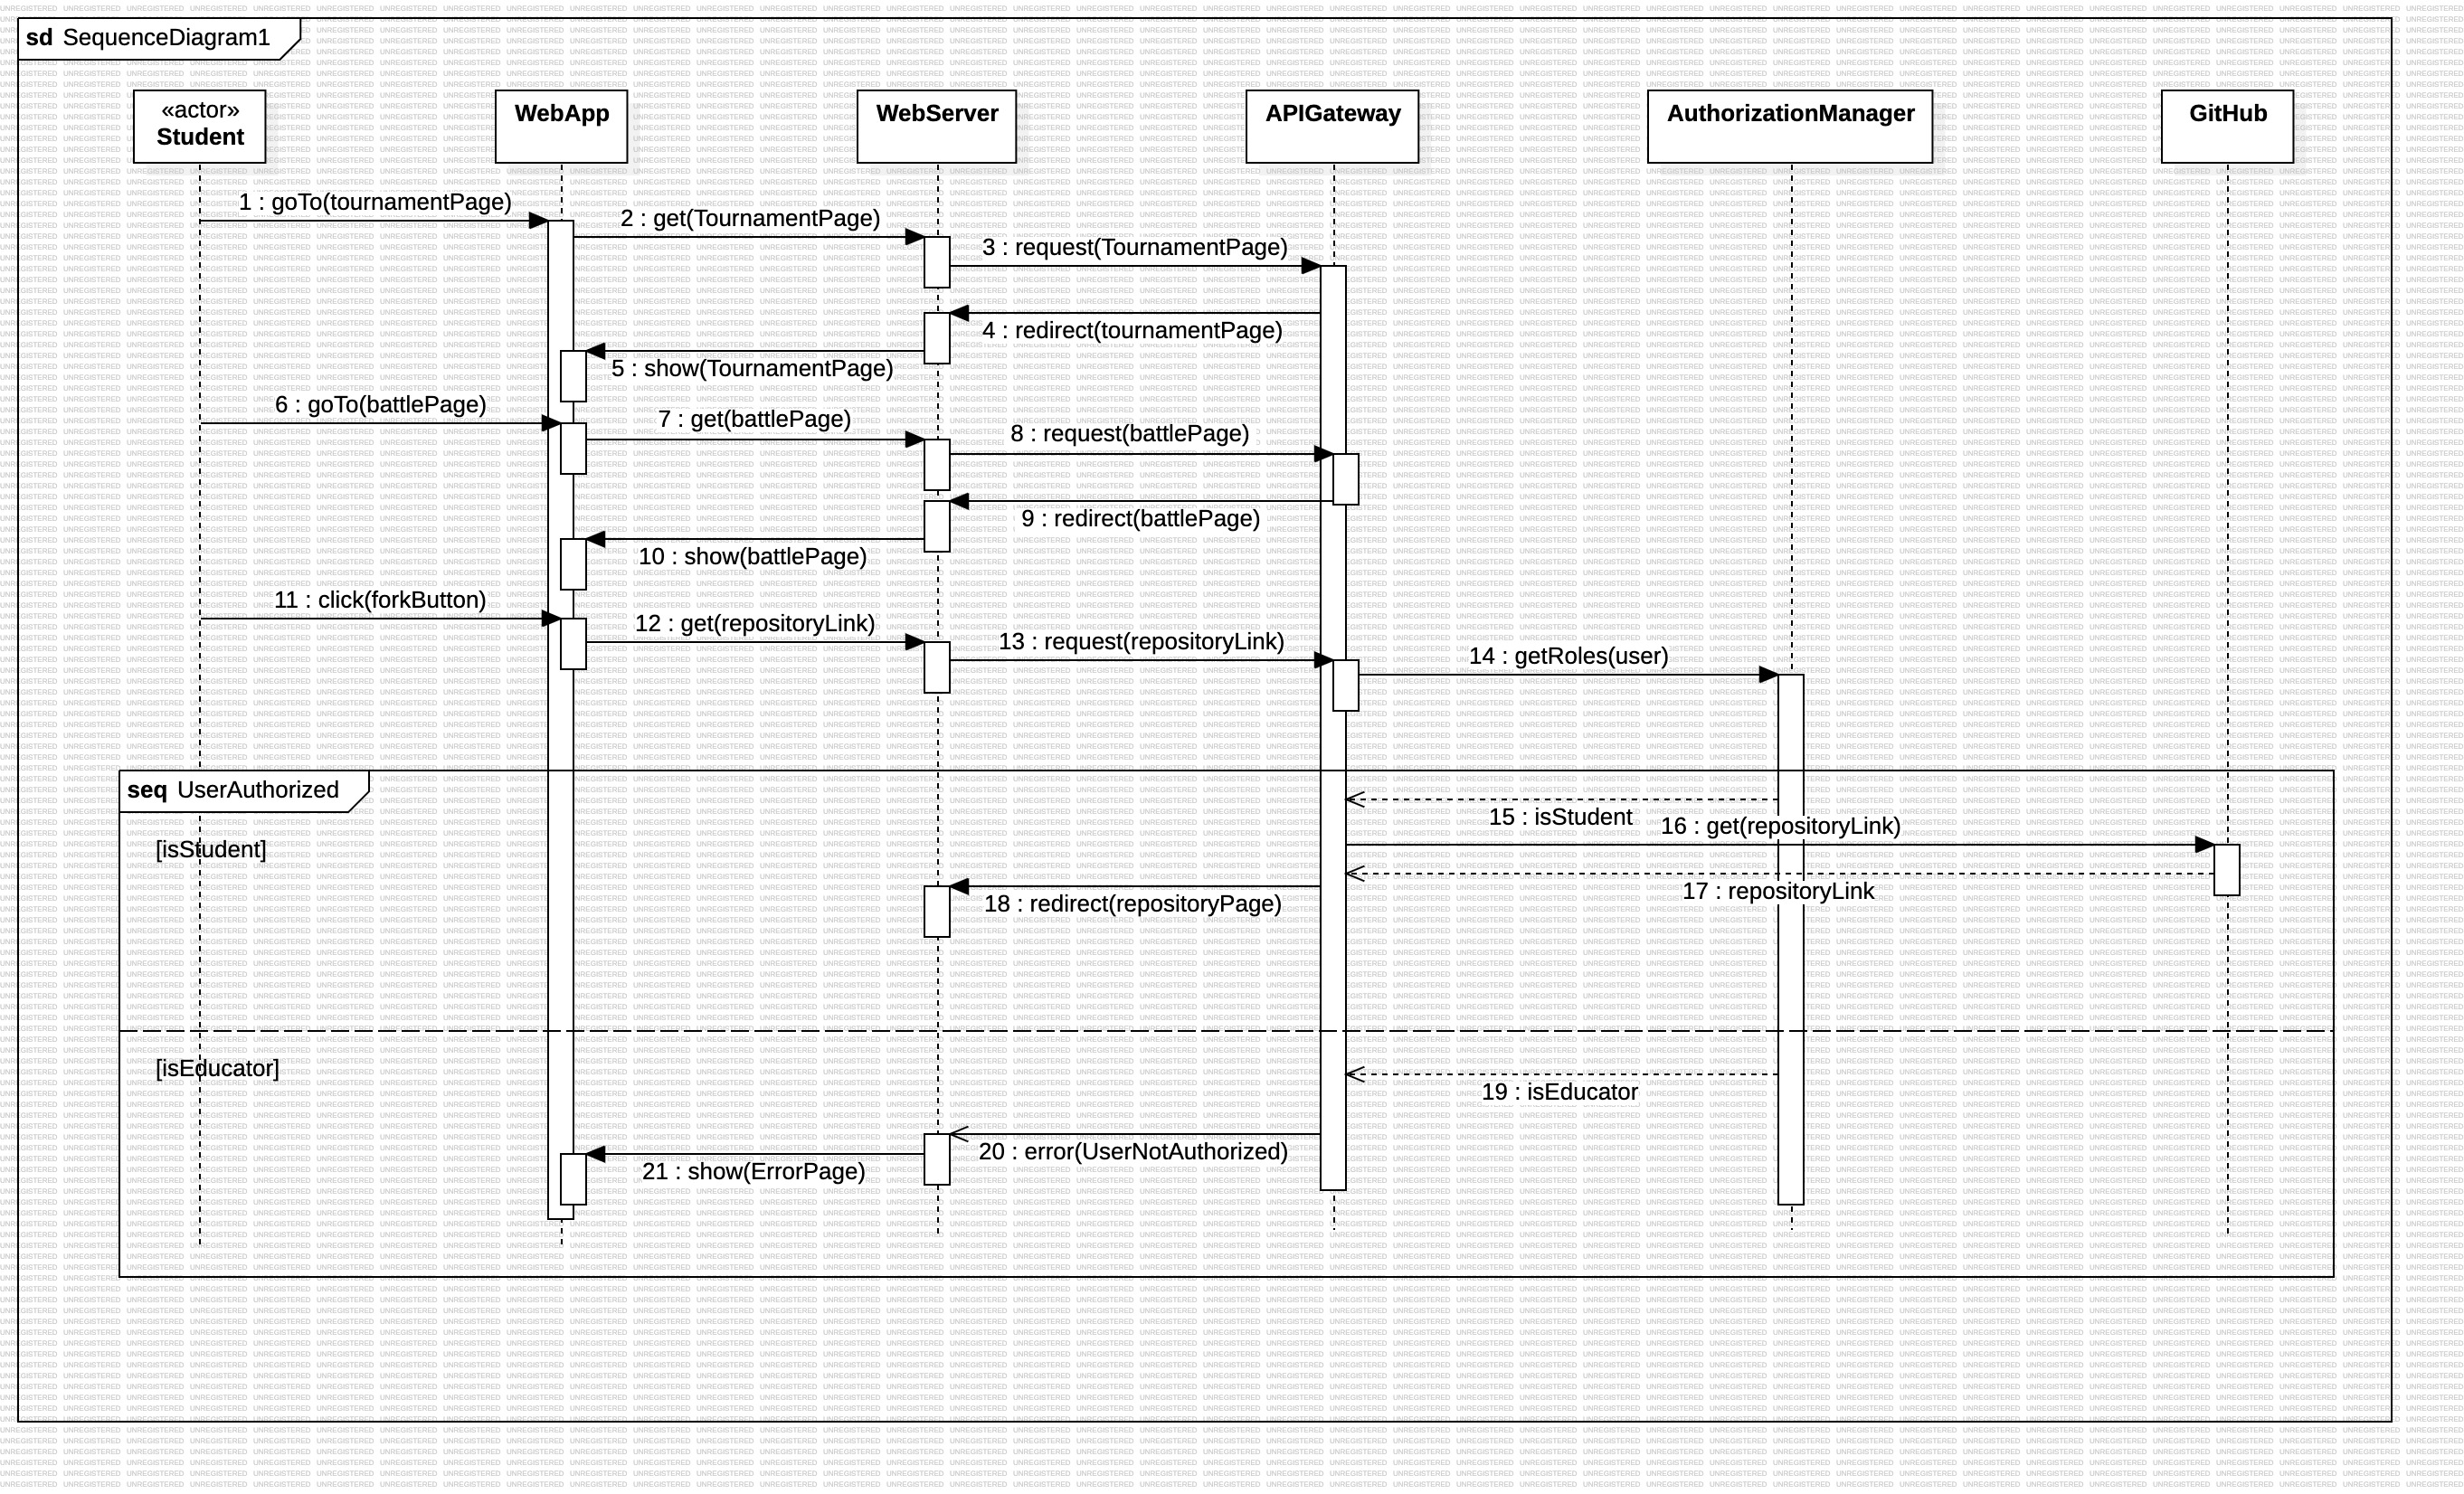
\includegraphics[width=\textwidth]{Diagrams/ForkRepositorySD.jpg}
    \caption{Runtime view}
\label{fig:runtime_view}
\end{figure}

\subsubsection*{Creation of a Team for a Battle}
\begin{figure}[H]
    \centering
    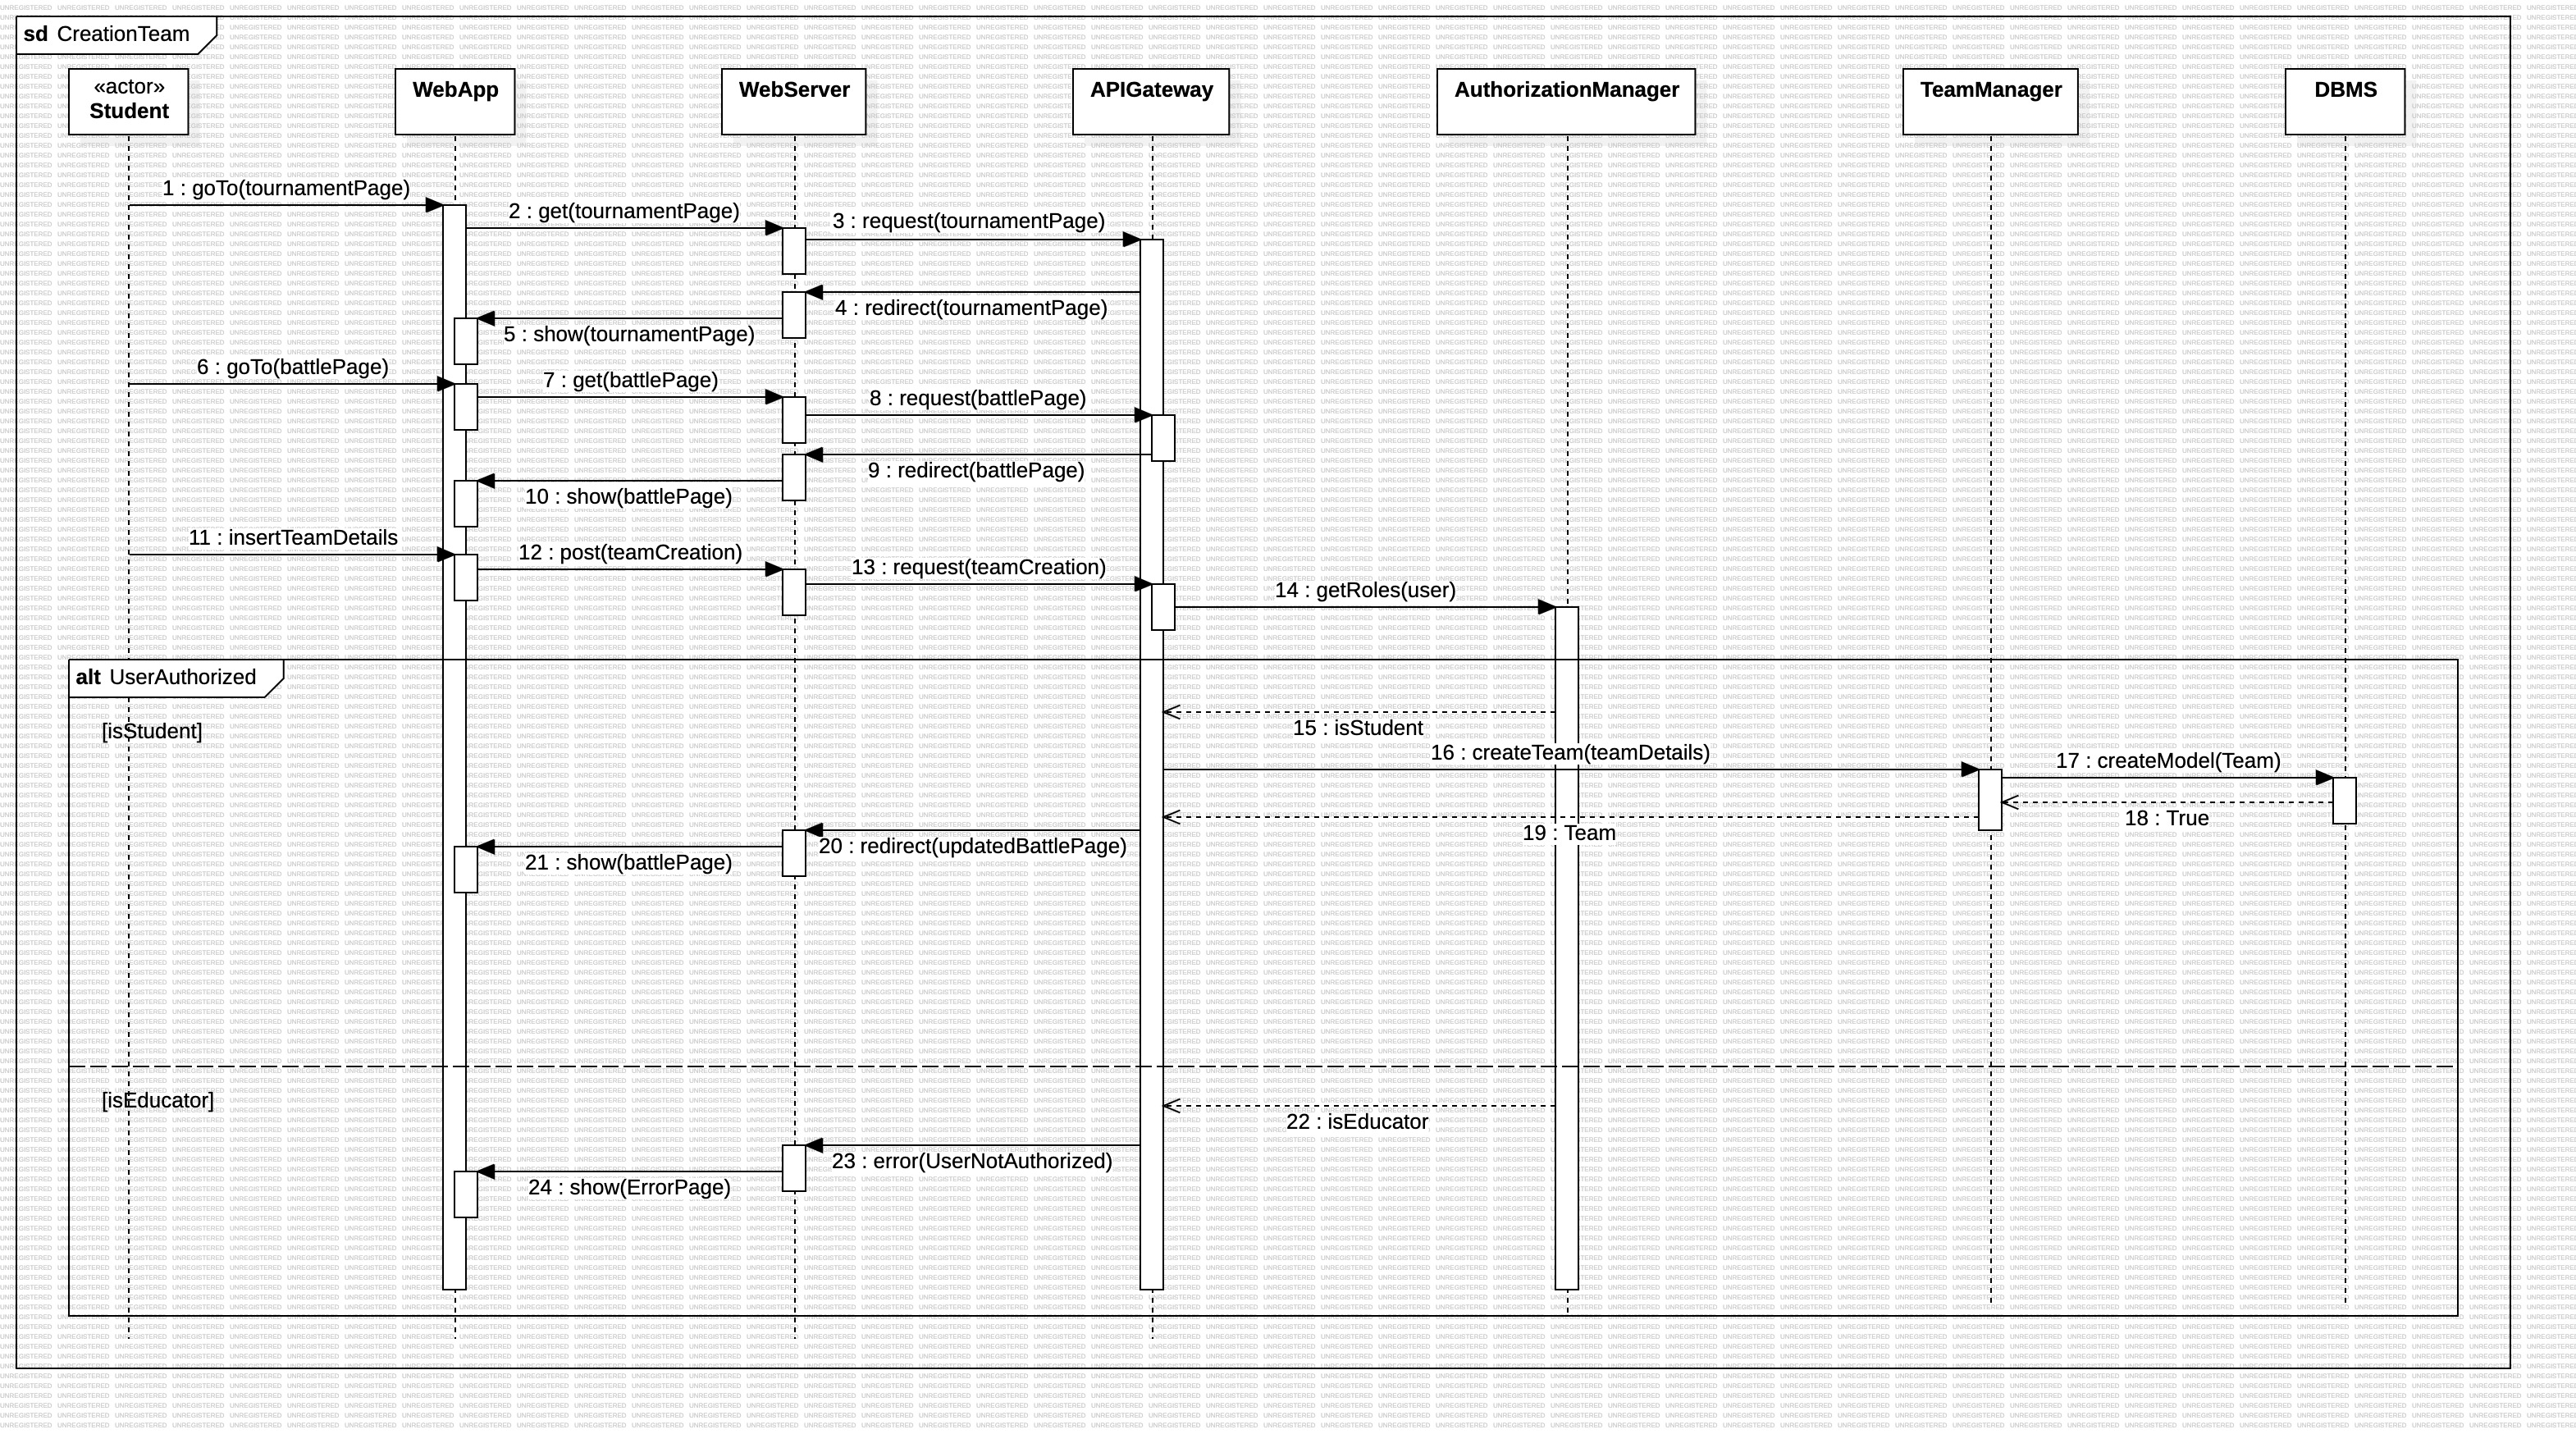
\includegraphics[width=\textwidth]{Diagrams/CreationTeamSD.jpg}
    \caption{Runtime view}
\label{fig:runtime_view}
\end{figure}
\clearpage
\subsection{Selected architectural styles and patterns}
\subsubsection{Three-tier architecture}
The three-tier architecture offers several key advantages of paramount importance for the CKB Platform:
\begin{enumerate}
    \item \textbf{Scalability}: by separating concerns into different layers, it becomes easier to scale each tier independently based on demand.
    \item \textbf{Maintainability}: modifications in one tier can be implemented without impacting the other tiers, simplifying maintenance and updates.
    \item \textbf{Flexibility}: Each tier can utilize the most suitable technologies, allowing for technological adaptability. For example: the presentation layer can adopt a frontend framework that best suits the needs of the application, while the application layer can adopt a backend framework that best suits the needs of the application.
    \item \textbf{Security}: Layer separation enables specific security measures at each level, enhancing overall protection. In the Figure\ \ref{fig:high_level_system} is shown that the different tier are physically connected through firewalls. This is a very important feature of the system since it allows to guarantee the security of the data.
    \item \textbf{Easier Testing and Debugging}: Individual layer testing and debugging lead to more efficient problem resolution. Different teams can work on different layers simultaneously, allowing for faster testing and debugging.
    \item \textbf{Improved Performance}: Effective load balancing across layers results in better overall system performance.
\end{enumerate}
\subsubsection{Model View Controller (MVC) pattern}
The Model-View-Controller (MVC) pattern is a software design paradigm that organizes an application into three interconnected components:

\begin{itemize}
    \item \textbf{Model:} Manages the data and business logic of the application.
    \item \textbf{View:} Responsible for the display and user interface.
    \item \textbf{Controller:} Acts as an intermediary between the Model and View, processing user input and responding to user interactions.
\end{itemize}
The MVC pattern is a good fit for the CKB Platform because as discussed above the platform is decomposed into three layer. In particular: the \textit{Model} is represented by the DBMS Component, the \textit{View} is represented by the WebApp Component and the WebServer subsystem. Finally the \textit{Controller} is represented by the Application Server Subsystem which implement several components such as the Login Manager, the Registration Manager, the Authorization Manager, the Evaluation Manager, the Ranking Manager, the Team Manager, the Submission Manager, the Invitation Manager, the Notification Manager, the Battle Manager and the Tournament Manager that are responsible to handle the data, process following the business logic and pass it to the \textit{View}. \\
Some of the benefits apported by the MVC to the CKB Platform are:

\begin{enumerate}
    \item \textbf{Modularity:} Separation of concerns allows for independent development, maintenance, and testing of each component.
    \item \textbf{Reusability:} Facilitates the reuse of components, especially the business logic encapsulated in the Model.
    \item \textbf{Scalability:} Makes scaling and updating the application more manageable as it grows in complexity.
    \item \textbf{Flexibility:} Each component can evolve independently, accommodating new technologies or changes in business requirements.
    \item \textbf{Improved Organization:} Enhances code readability and maintainability due to its structured organization.
    \item \textbf{Simplified Collaboration:} Enables different development teams to work on each component without overlap, improving collaborative efforts.
\end{enumerate}

\subsubsection{Facade pattern}
The Facade pattern is a structural design pattern that provides a simplified interface to a complex system. It hides the complexities of the system and provides an interface to the client from where the client can access the system.
This patterns comes handy in the CKB platform system because it allows the web server to communicate only with one component, the \textit{APIGateway}, which is responsible to dispatch the requests to the correct component inside the Application Server Subsystem.
\subsubsection{Observer pattern}
The Observer pattern is a behavioral design pattern that allows an object, called the subject, to notify other objects, called observers, when its state changes. The Observer pattern provides a way to subscribe and unsubscribe to and from these events for any object that implements a subscriber interface. In the context of CKB platform, it is used to notify the users when a new notification is available. The \textit{Notification Manager} is the subject and the \textit{WebApp} is the observer. The \textit{WebApp} subscribes to the \textit{Notification Manager} and it is notified when a new notification is available. Also another use case of this pattern is when \textit{GitHub} is the subject and the \textit{Evaluation Manager} is the observer. In this case the \textit{Evaluation Manager} subscribes to GitHub and it is notified when a new submission is available.
\subsection{Other design decisions}
In this section are shown other design decisions that were taken during the design phase of the system.
\subsubsection{Document-oriented database}
The CKB Platform data architecture does not require complex relationships between data entities. The data is stored in a hierarchical format, which is well-suited for document-oriented databases. The data is stored in JSON format, which is useful when passing data to a fronted framework based Webapp as in the case of CKB Platform. Moreover the use of a document-oriented database provides several benefits:
\begin{itemize}
\item \textbf{Scalability}: The ability to scale is paramount in our system's design. Document-oriented databases excel in providing both horizontal and vertical scalability. This scalability is essential for our application, given the expected growth in data and user traffic. The distribution of data across multiple servers or nodes is seamlessly managed, ensuring consistent performance and robustness.
\item \textbf{Performance}: The speed and performance of document-oriented databases are noteworthy. Their design is optimized for quick data retrieval, especially in scenarios involving large volumes of data and simple queries. This is achieved through efficient data storage and retrieval mechanisms, which is crucial for maintaining a high level of responsiveness in our application.
\item \textbf{Developer Productivity}: The alignment of document-oriented databases with modern development practices significantly enhances developer productivity. The use of a JSON-like format reduces the complexity of data handling and increases the ease of development, as it closely resembles the data structures used in programming languages.
\item \textbf{Real-Time Analytics}: The ability to perform real-time analytics is an important feature for the CKB Platform, since it handles evaluation and ranking of students. Document-oriented databases are well-suited for this purpose, as they can process large volumes of data in real-time.
\end{itemize}

\subsubsection{Data Storage}
The CKB Platform split the data storage into two main components. The business relative data, such as Users, Tournaments and Battles, is stored in a document-oriented database. The files relative to the CodeKata, such as the tests and the automation scripts and as well as the submissions of the Teams, are stored in GitHub repositories. This choice was made in order to avoid duplication and any mismatch of data. In fact, the files relative to the CodeKata are already stored in GitHub repositories, so it is not necessary to store them also in the document-oriented database. The same reasoning goes also for the submission of the Teams, since there could be multiple version of the same file that GitHub will take care of. Moreover, the use of GitHub repositories allows to easily manage the submissions of the Teams. In fact, the submissions are stored in the repositories of the Teams and the evaluation is triggered by the GitHub Action. GitHub also offers APIs that allow to easily manage the repositories.

\subsubsection{Automatic Evaluation}
The component that handles the Automatic Evaluation, \textit{Evaluation Manager}, should be containerized to cope with spikes of submission requests and so their respective evaluation processes that could occupy a significant amount of processing resources. The containerization of the component allows to easily scale the component horizontally by adding more instances of the container as the requests grow in number.